
\chapter{Results}

The algorithms have been evaluated with 1120 mono sounds from the test dataset for the Kaggle Audio tagging competition created by \\
the MTG and Freesound. The test set for the dataset is an accurate representation of the content of the whole dataset for the competition. \\
The dataset has been manually anotated by the author using the script evaluation.py in the Evaluation folder on thew github repository. \\
The evaluation was carried by annotating the existance of the following problems: Hum, Clicks, Noise Bursts, Saturation and Silence. \\
Other algorithms that had to be evaluated were Phase issues. However, as the dataset is formed exclusively of mono files, the algorithms were not properly evaluated.

\section{Hum detection evaluation}
Four parameters of the essentia Hum algorithm were considered in the evaluation: TimeWindow, minimumDuration, NumberofHarmonics and timeContinuity.

\begin{figure}[!ht]
	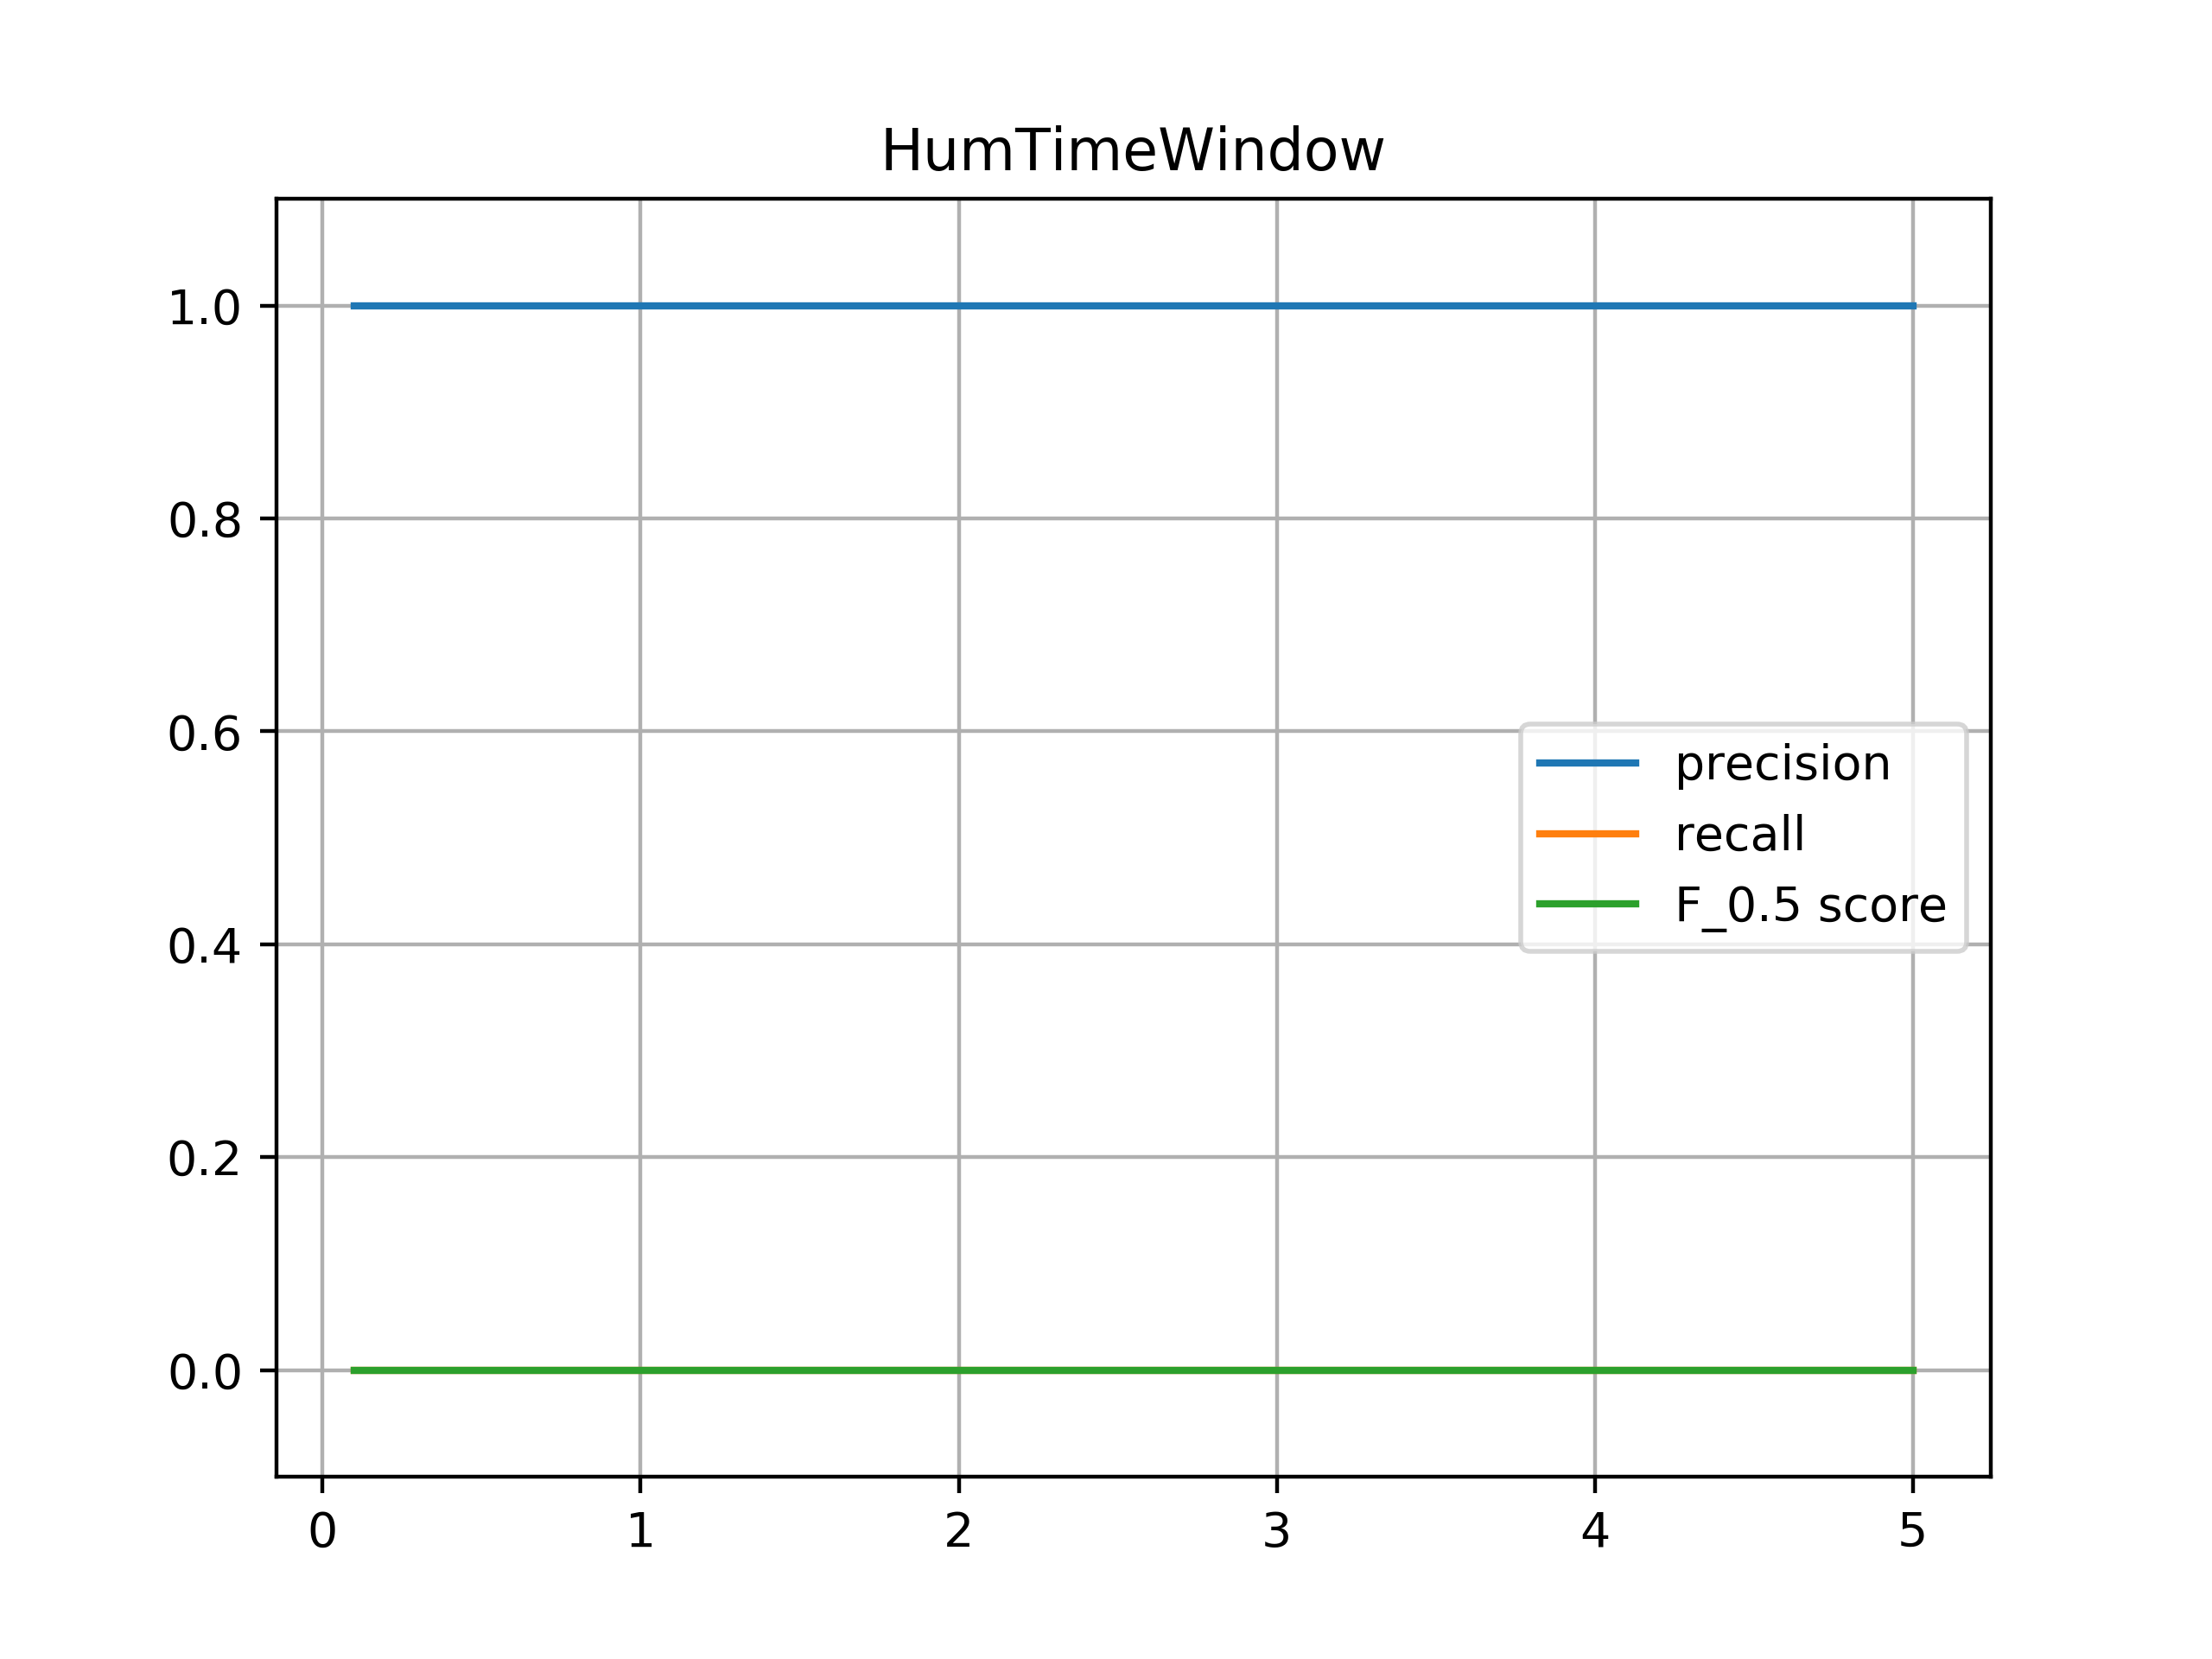
\includegraphics[clip,width=\columnwidth]{Figures/HumTimeWindow.png}% 
	\caption{timeWindow parameter sweep results (accuracy, F score and recall)}
	\label{fig:humTimeWindow}
\end{figure}

\begin{figure}[!ht]
	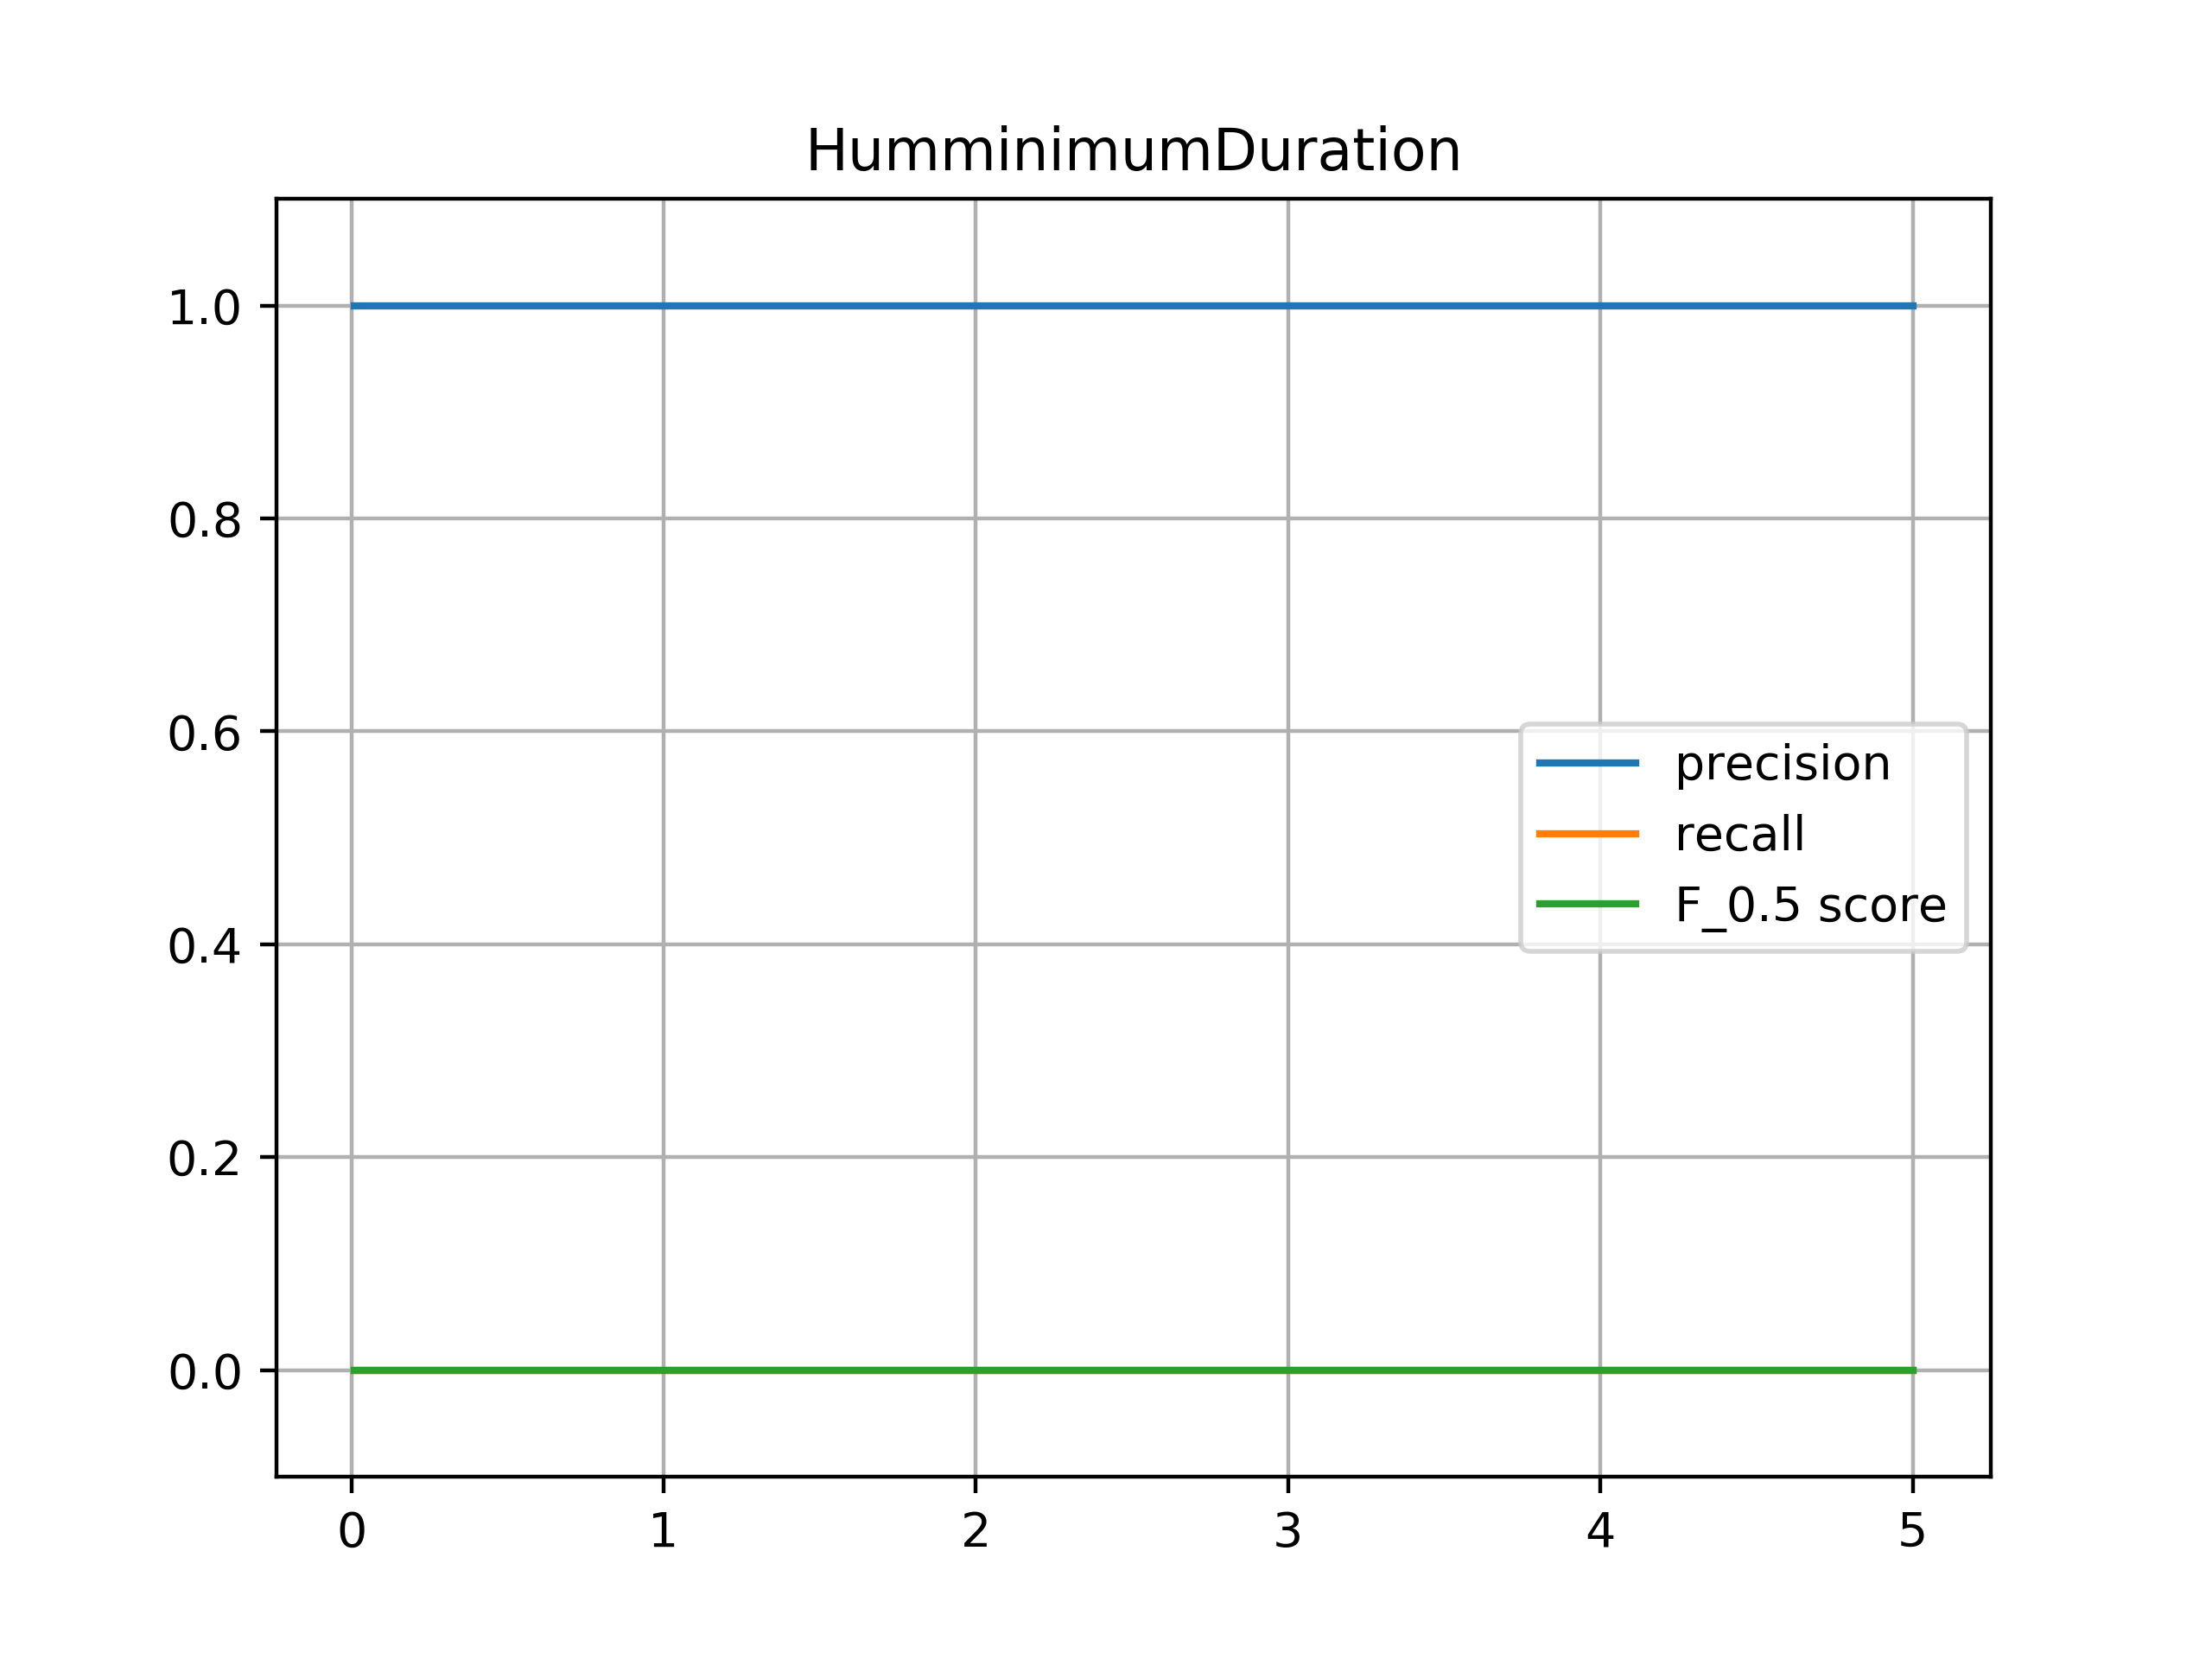
\includegraphics[clip,width=\columnwidth]{Figures/HumminimumDuration.png}% 
	\caption{minimumDuration parameter sweep results (accuracy, F score and recall)}
	\label{fig:humminimumDuration}
\end{figure}

\begin{figure}[!ht]
	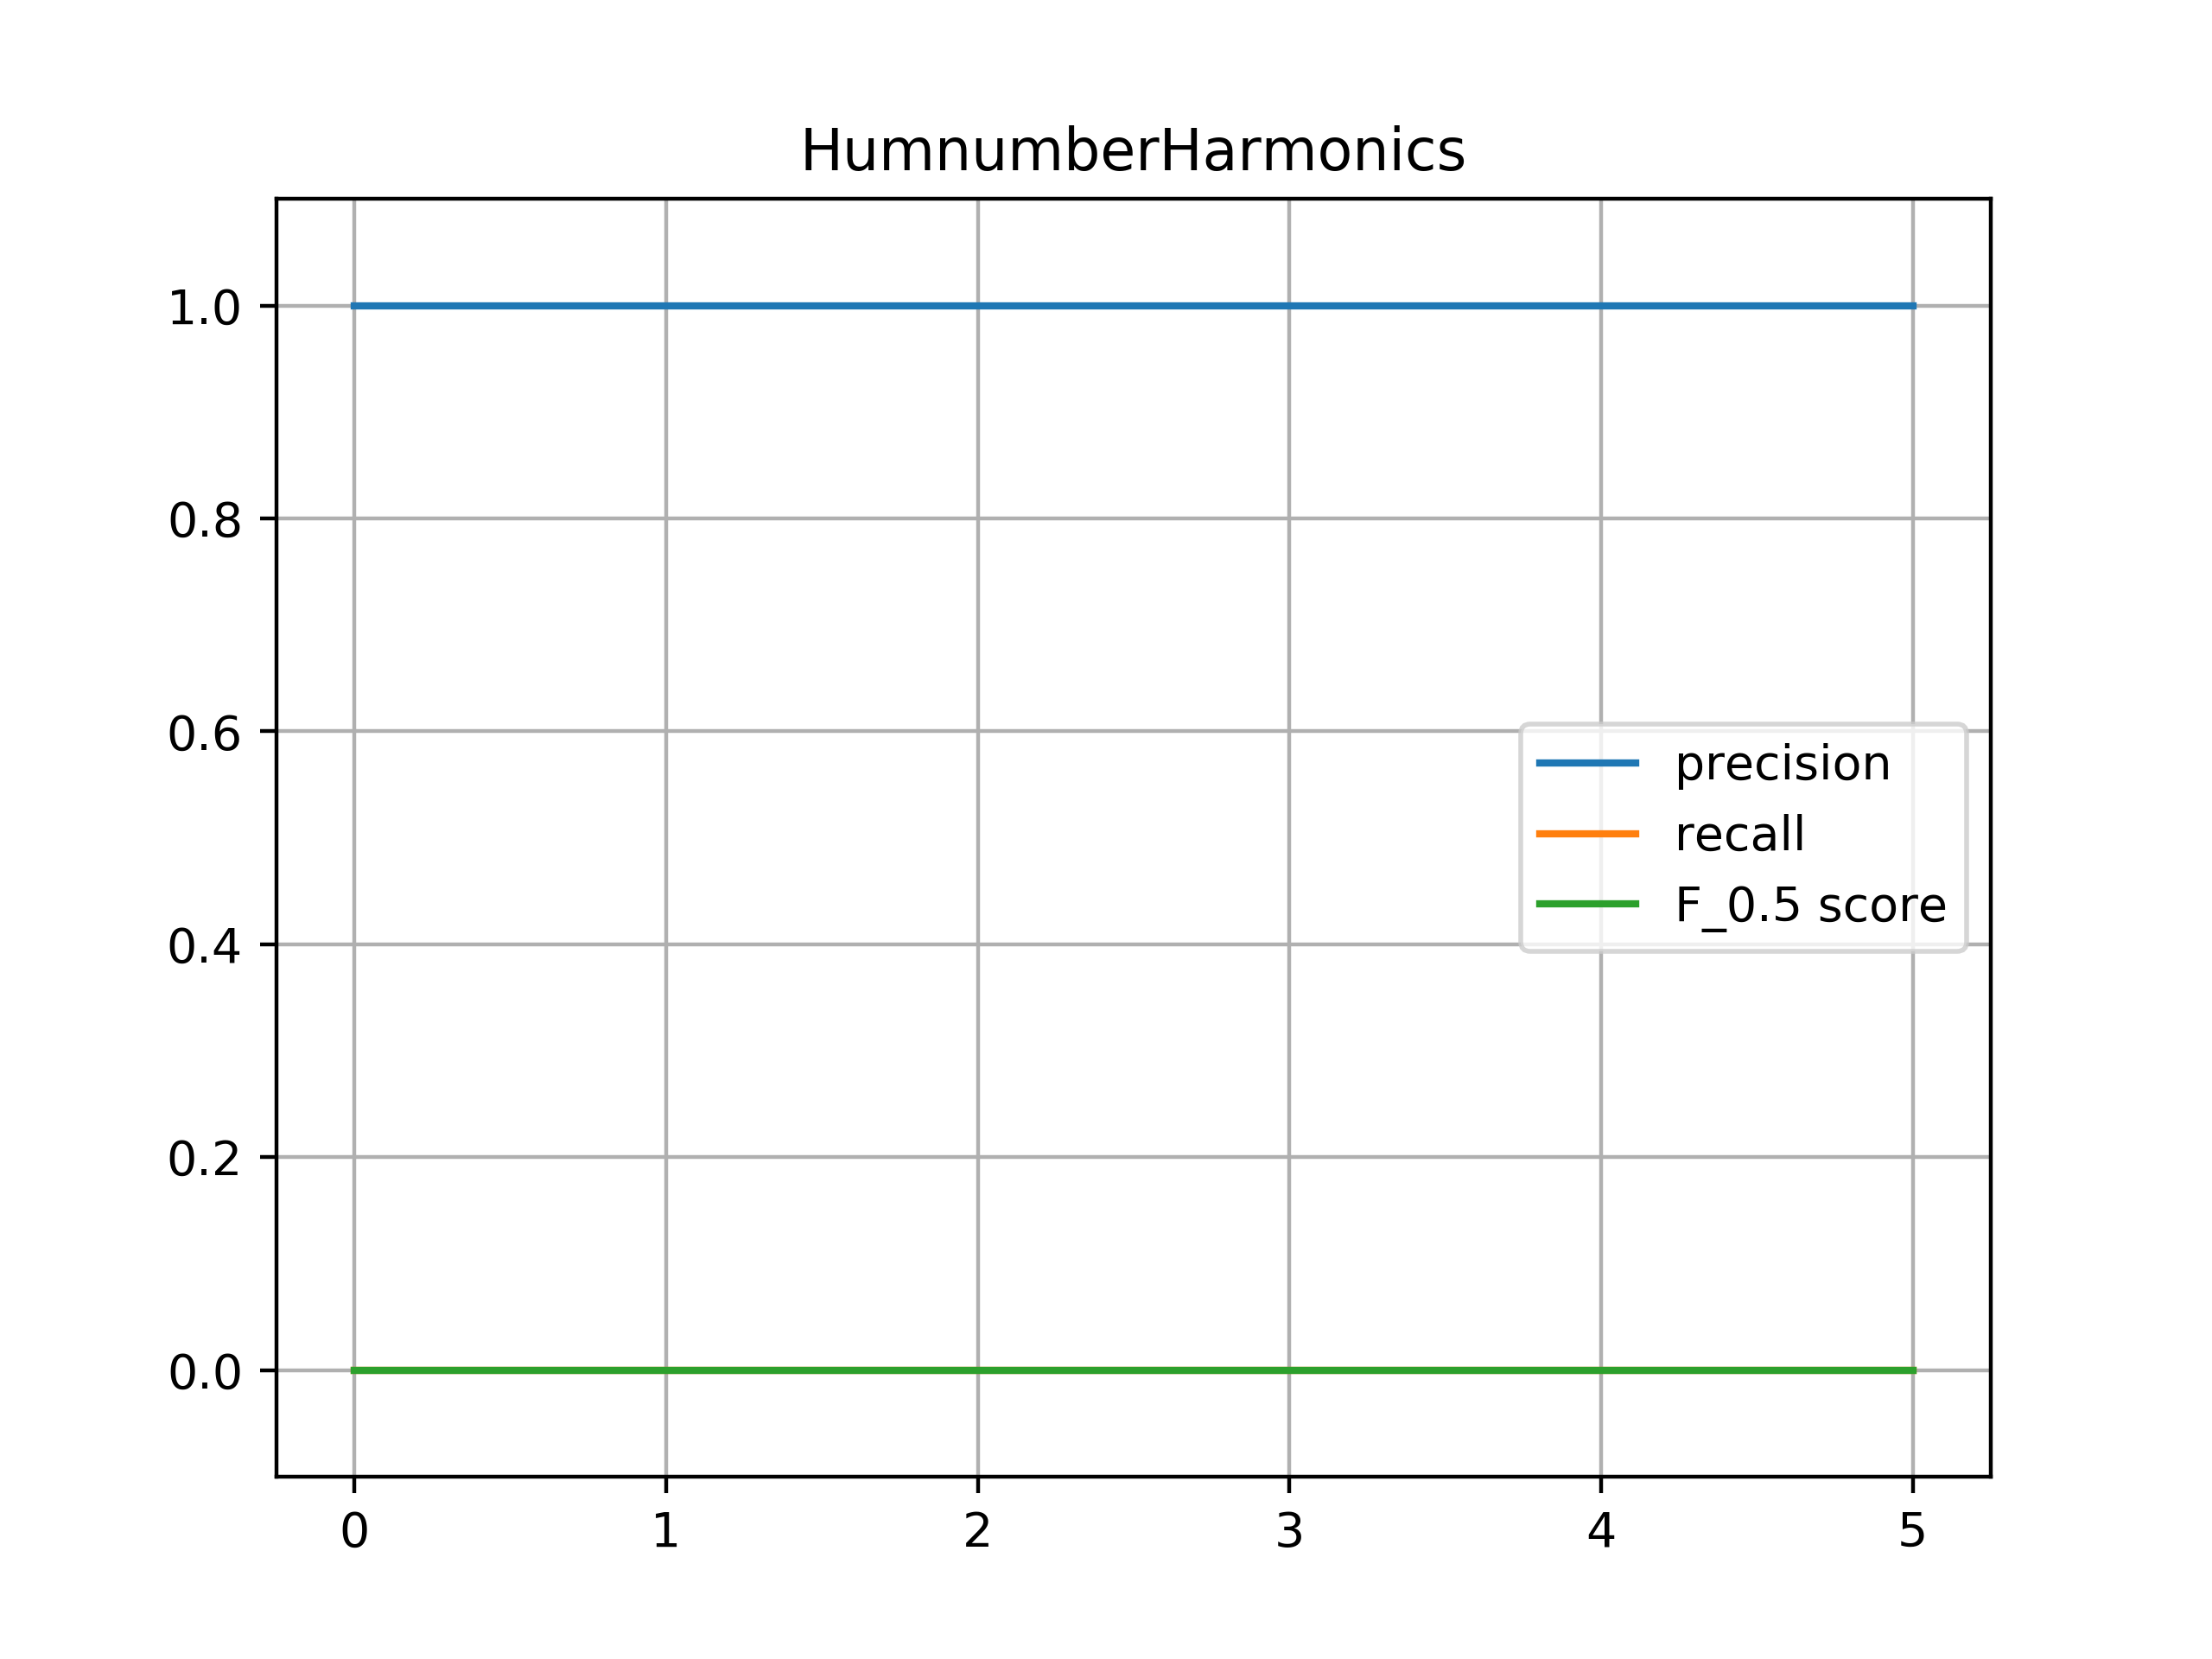
\includegraphics[clip,width=\columnwidth]{Figures/HumnumberHarmonics.png}% 
	\caption{numberHarmonics parameter sweep results (accuracy, F score and recall)}
	\label{fig:humnumberHarmonics}
\end{figure}

\begin{figure}[!ht]
	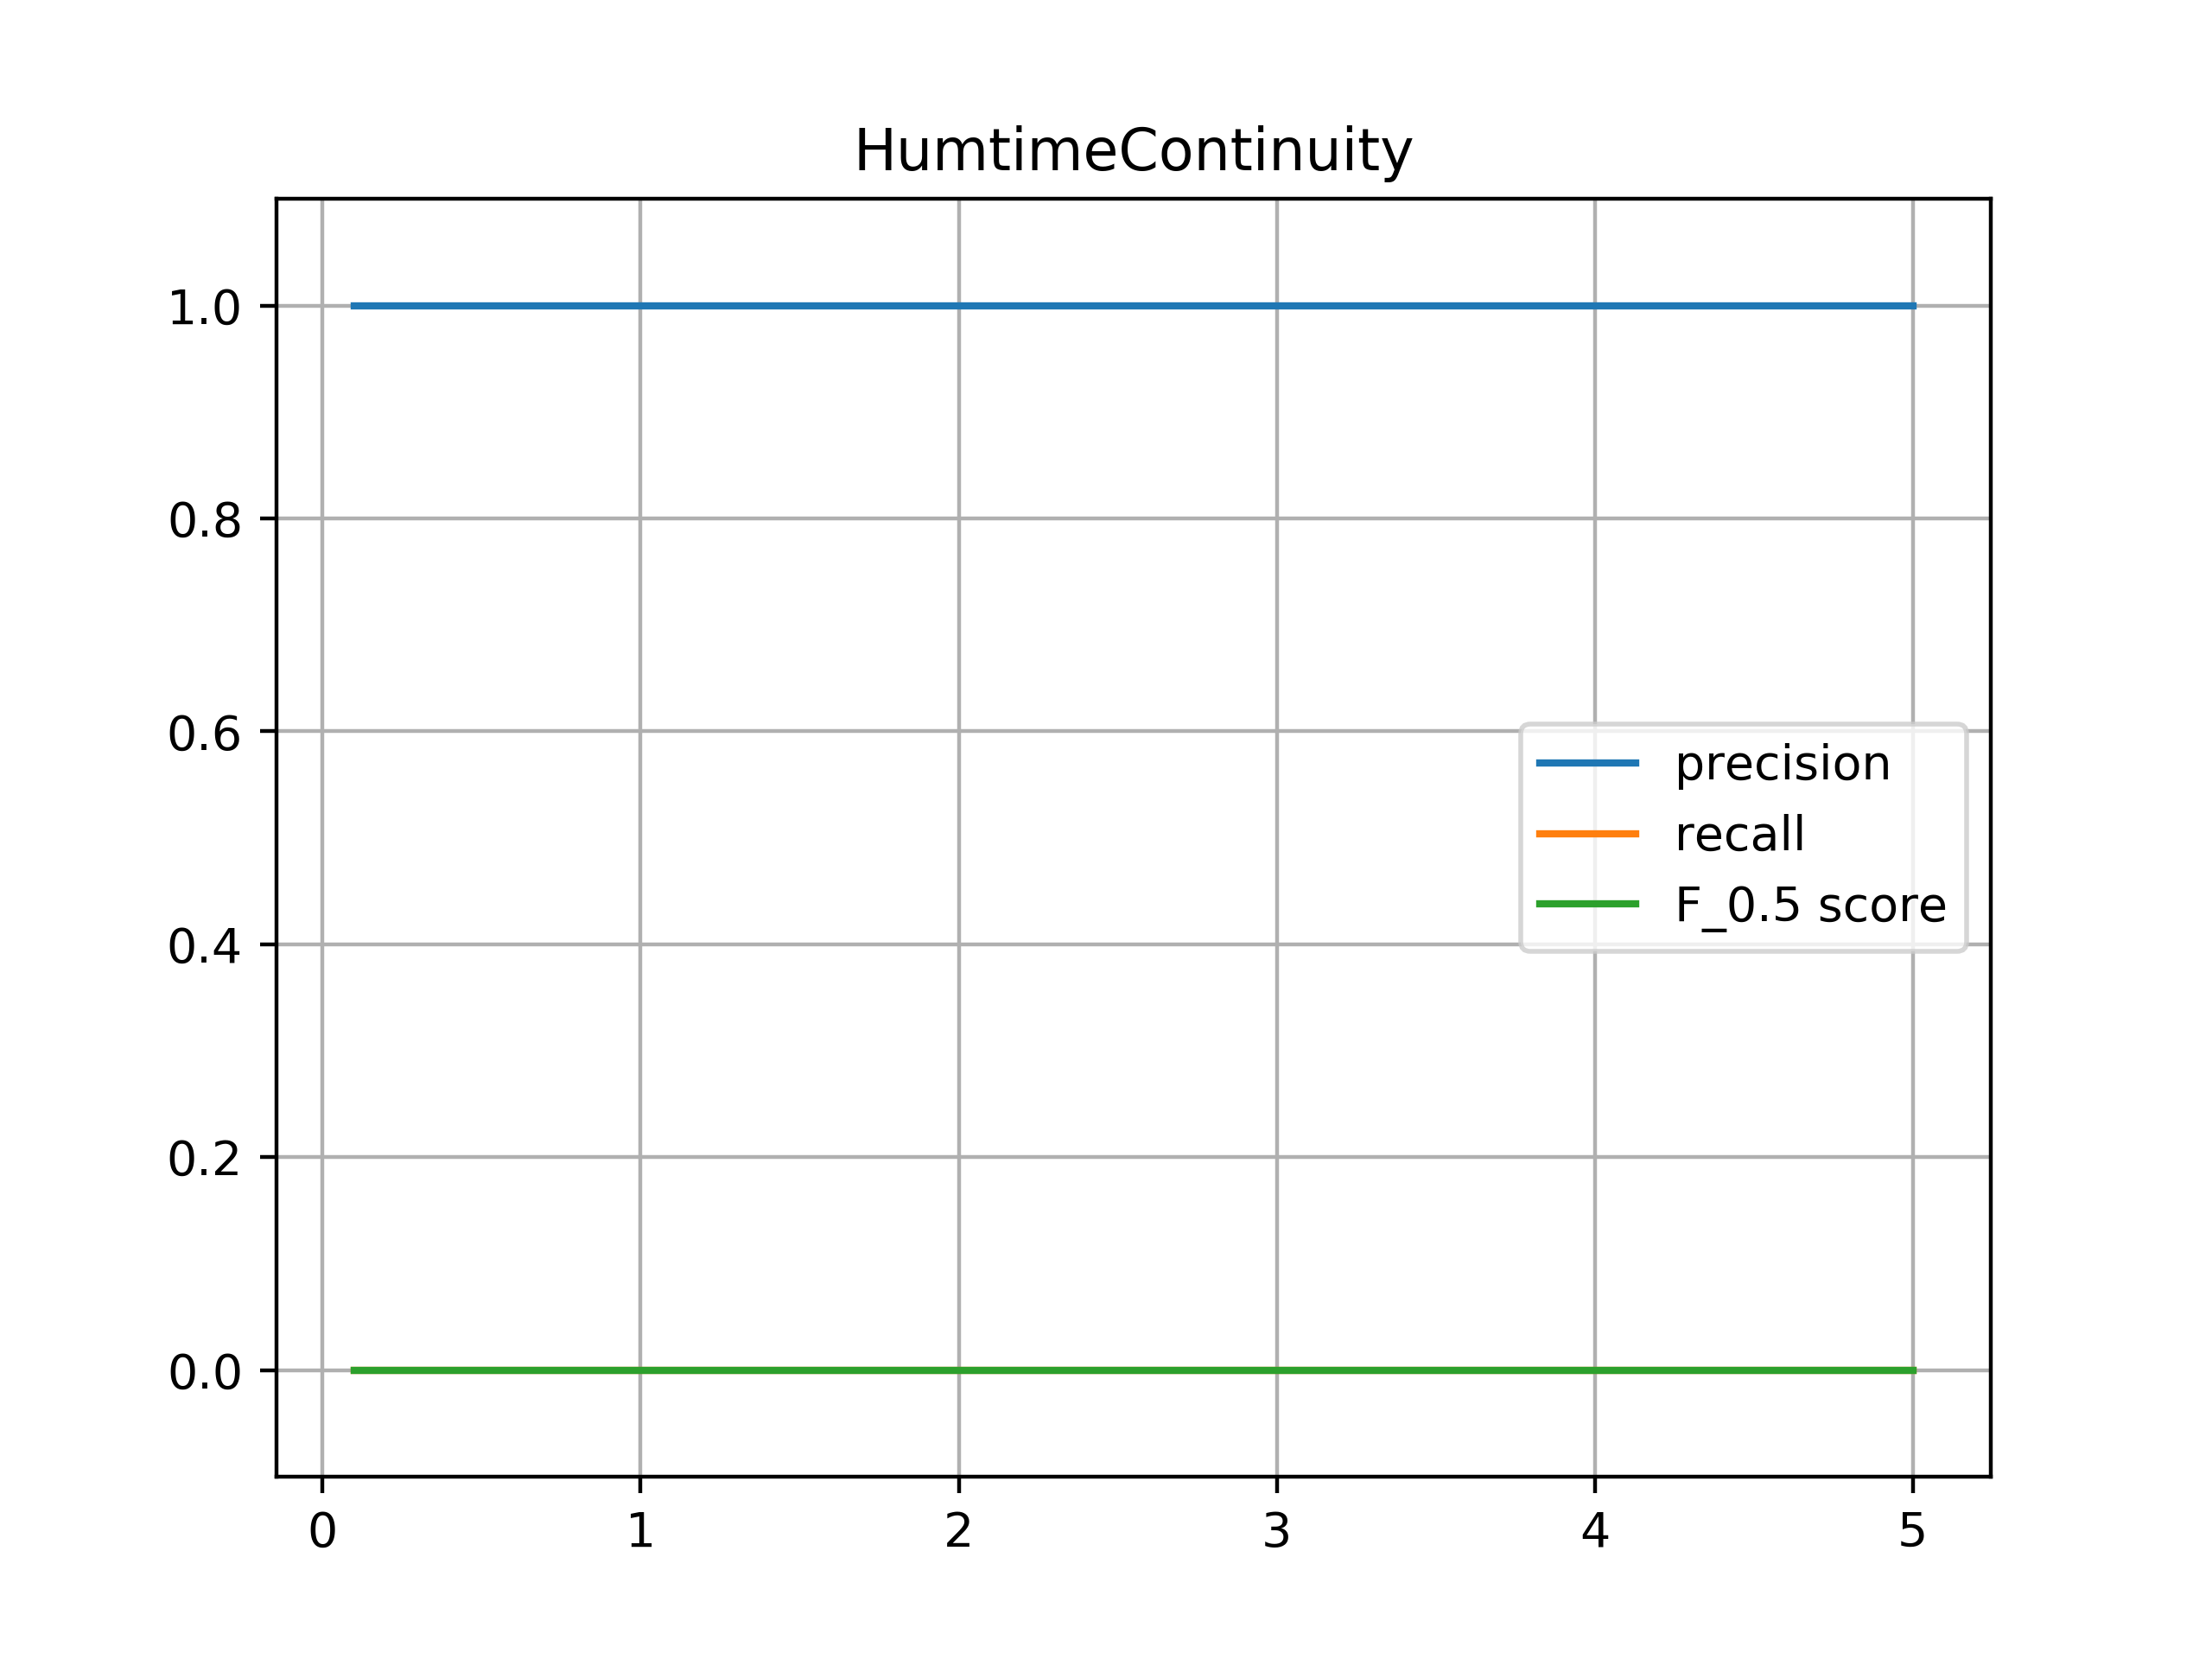
\includegraphics[clip,width=\columnwidth]{Figures/HumtimeContinuity.png}% 
	\caption{timeContinuity parameter sweep results (accuracy, F score and recall)}
	\label{fig:humtimeContinuity}
\end{figure}

\begin{figure}[!ht]
	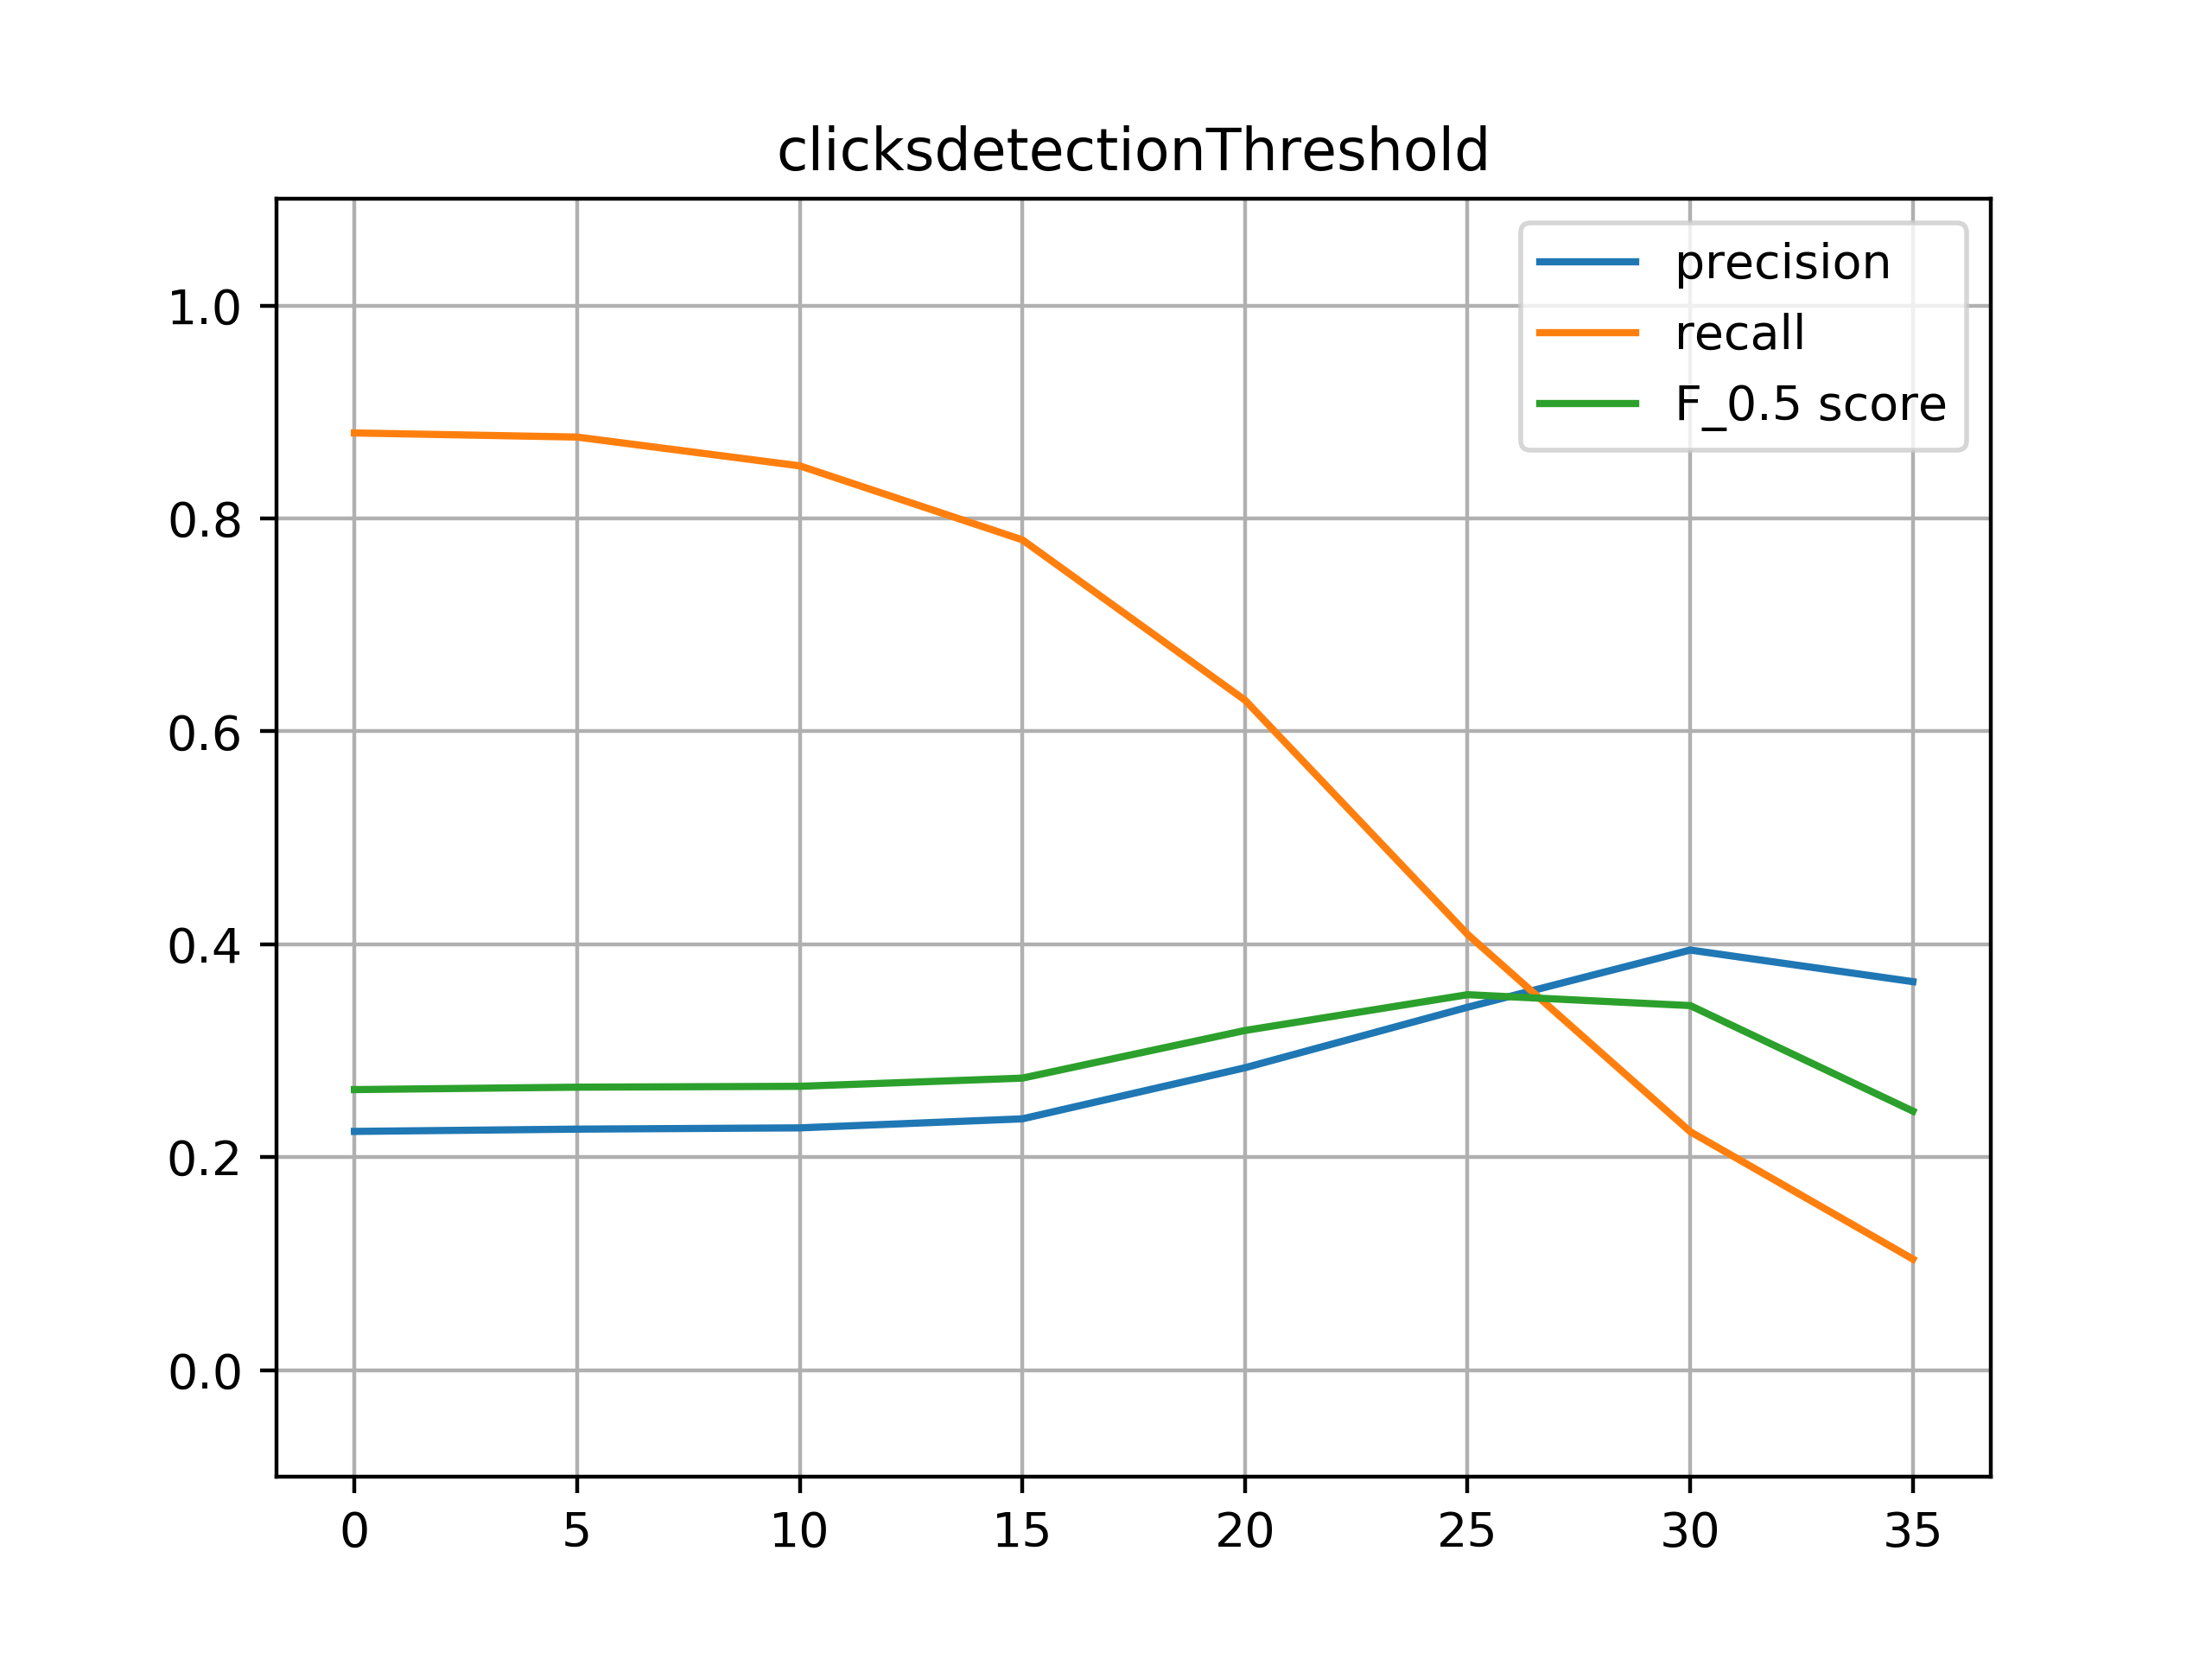
\includegraphics[clip,width=\columnwidth]{Figures/clicksdetectionThreshold.png}% 
	\caption{detectionThreshold parameter sweep results (accuracy, F score and recall)}
	\label{fig:clicksdetectionThreshold}
\end{figure}

\begin{figure}[!ht]
	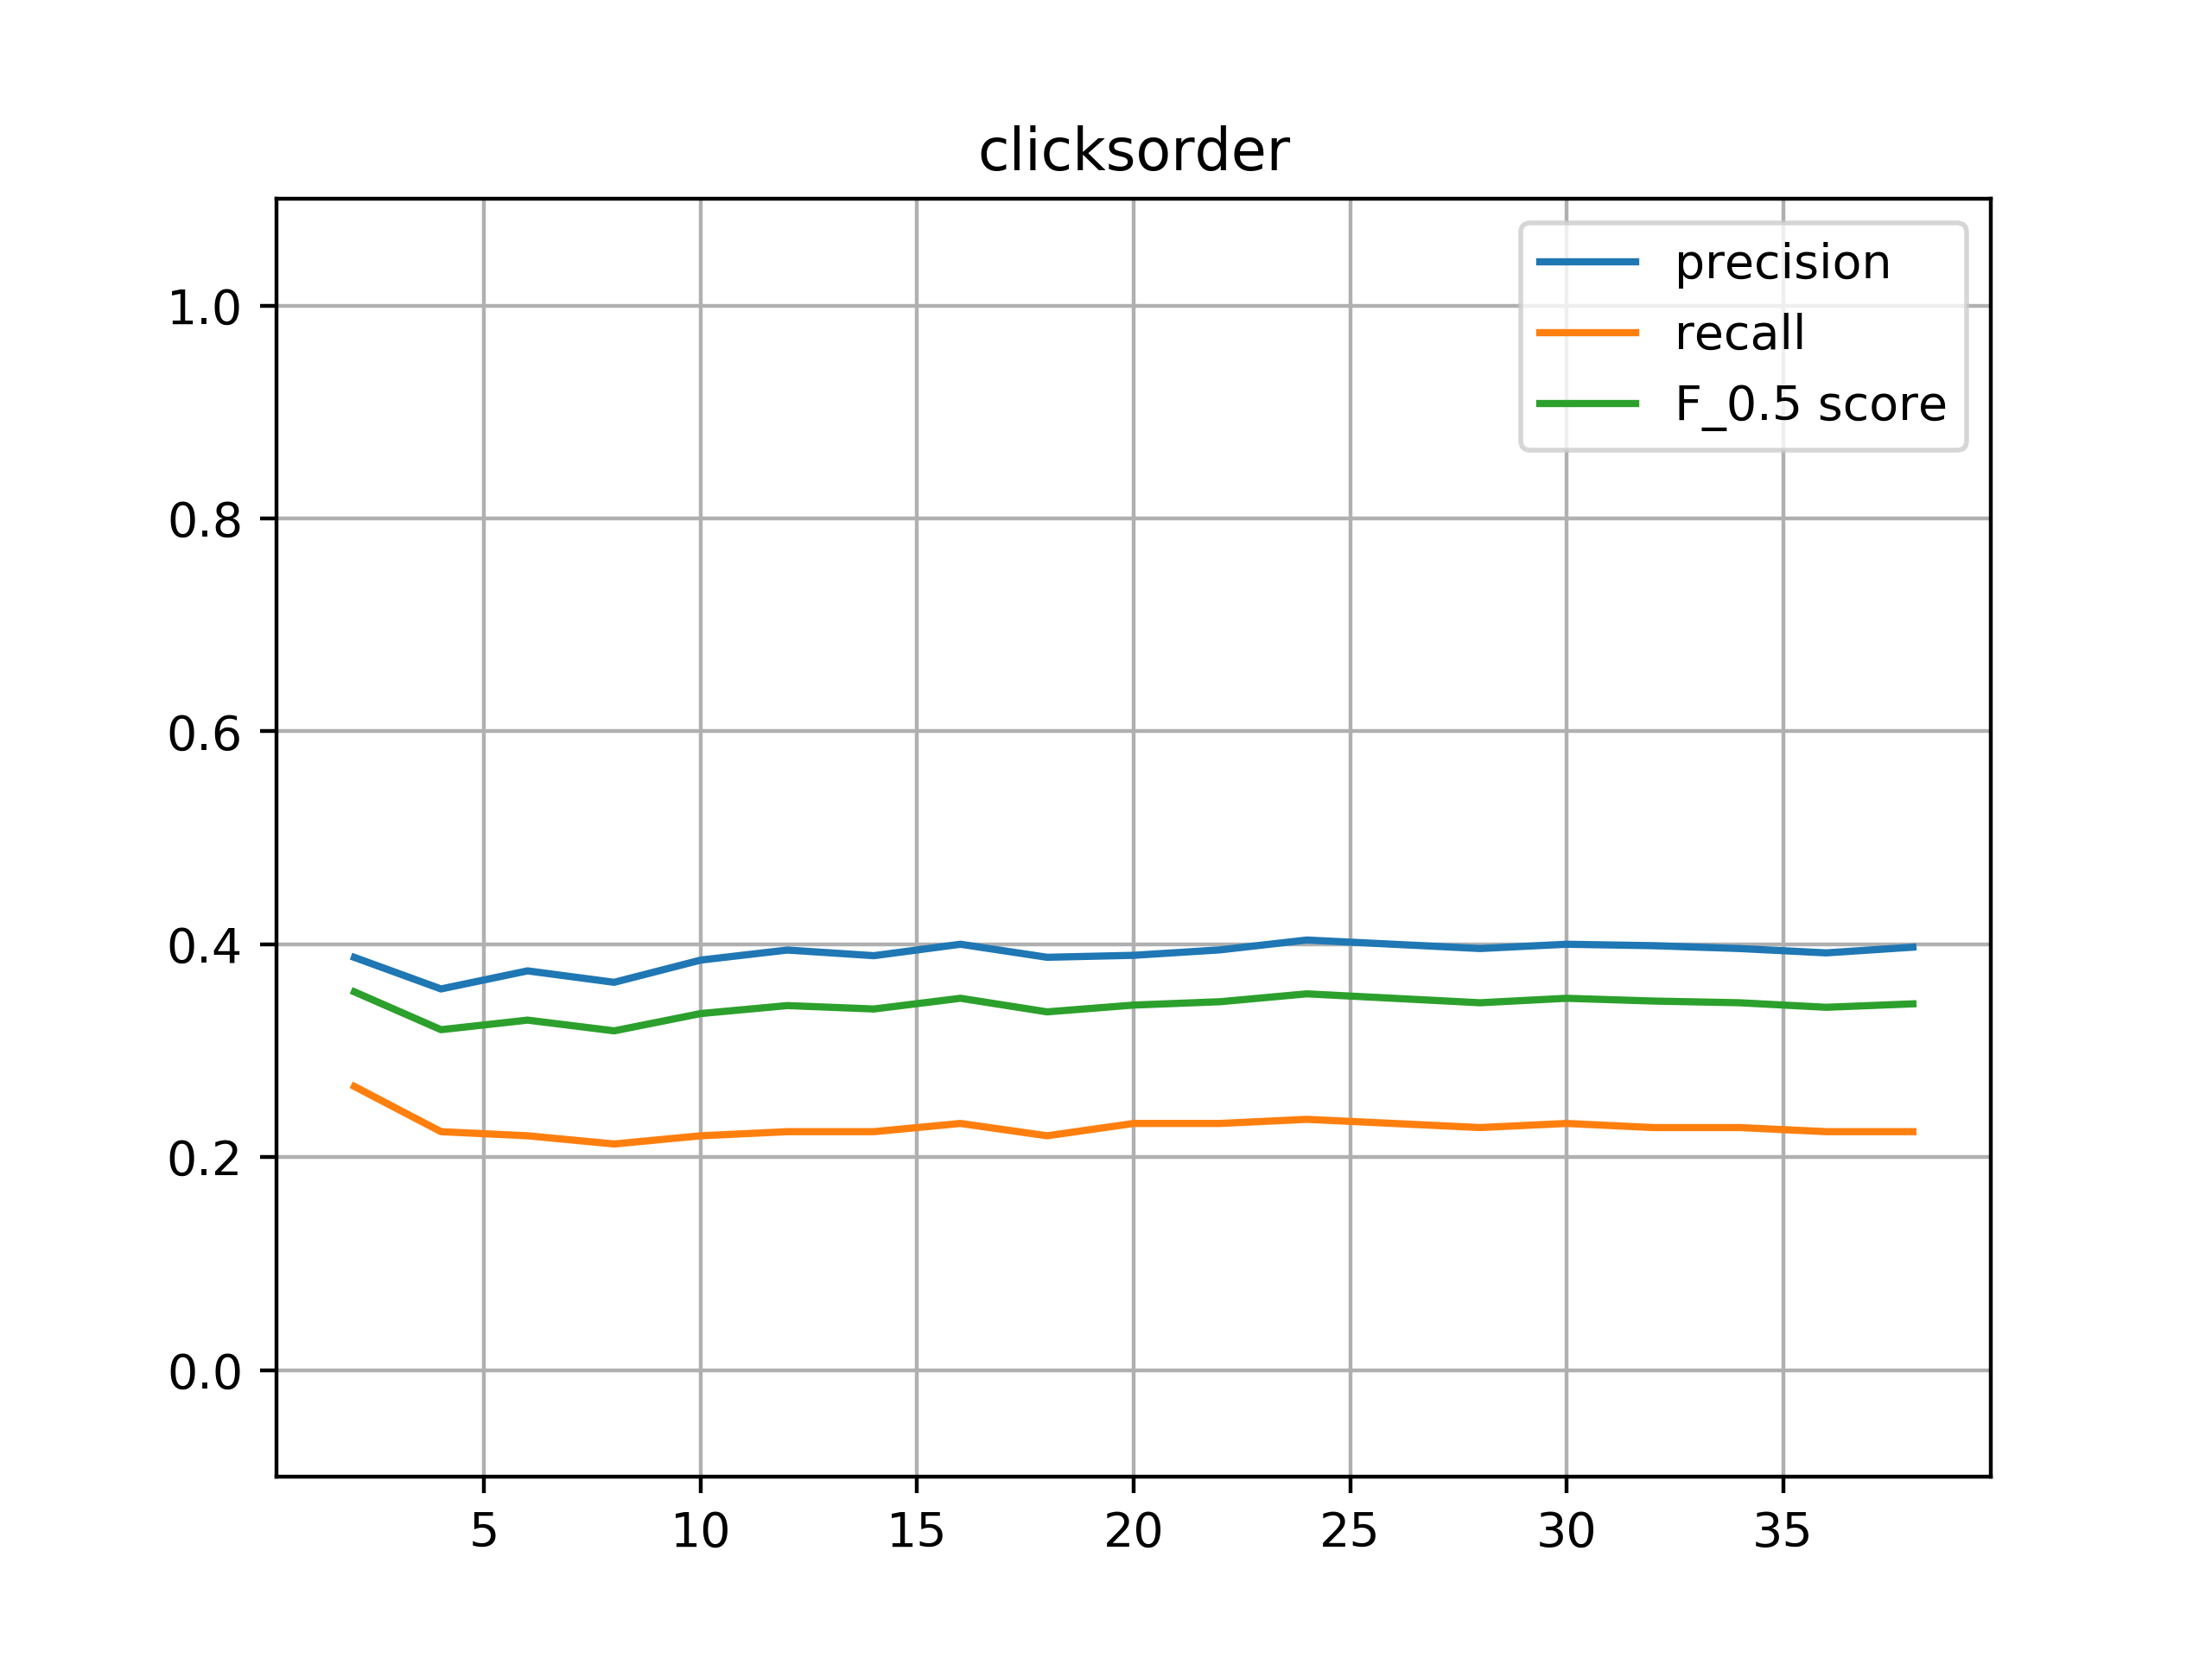
\includegraphics[clip,width=\columnwidth]{Figures/clicksorder.png}% 
	\caption{order parameter sweep results (accuracy, F score and recall)}
	\label{fig:clicksorder}
\end{figure}

\begin{figure}[!ht]
	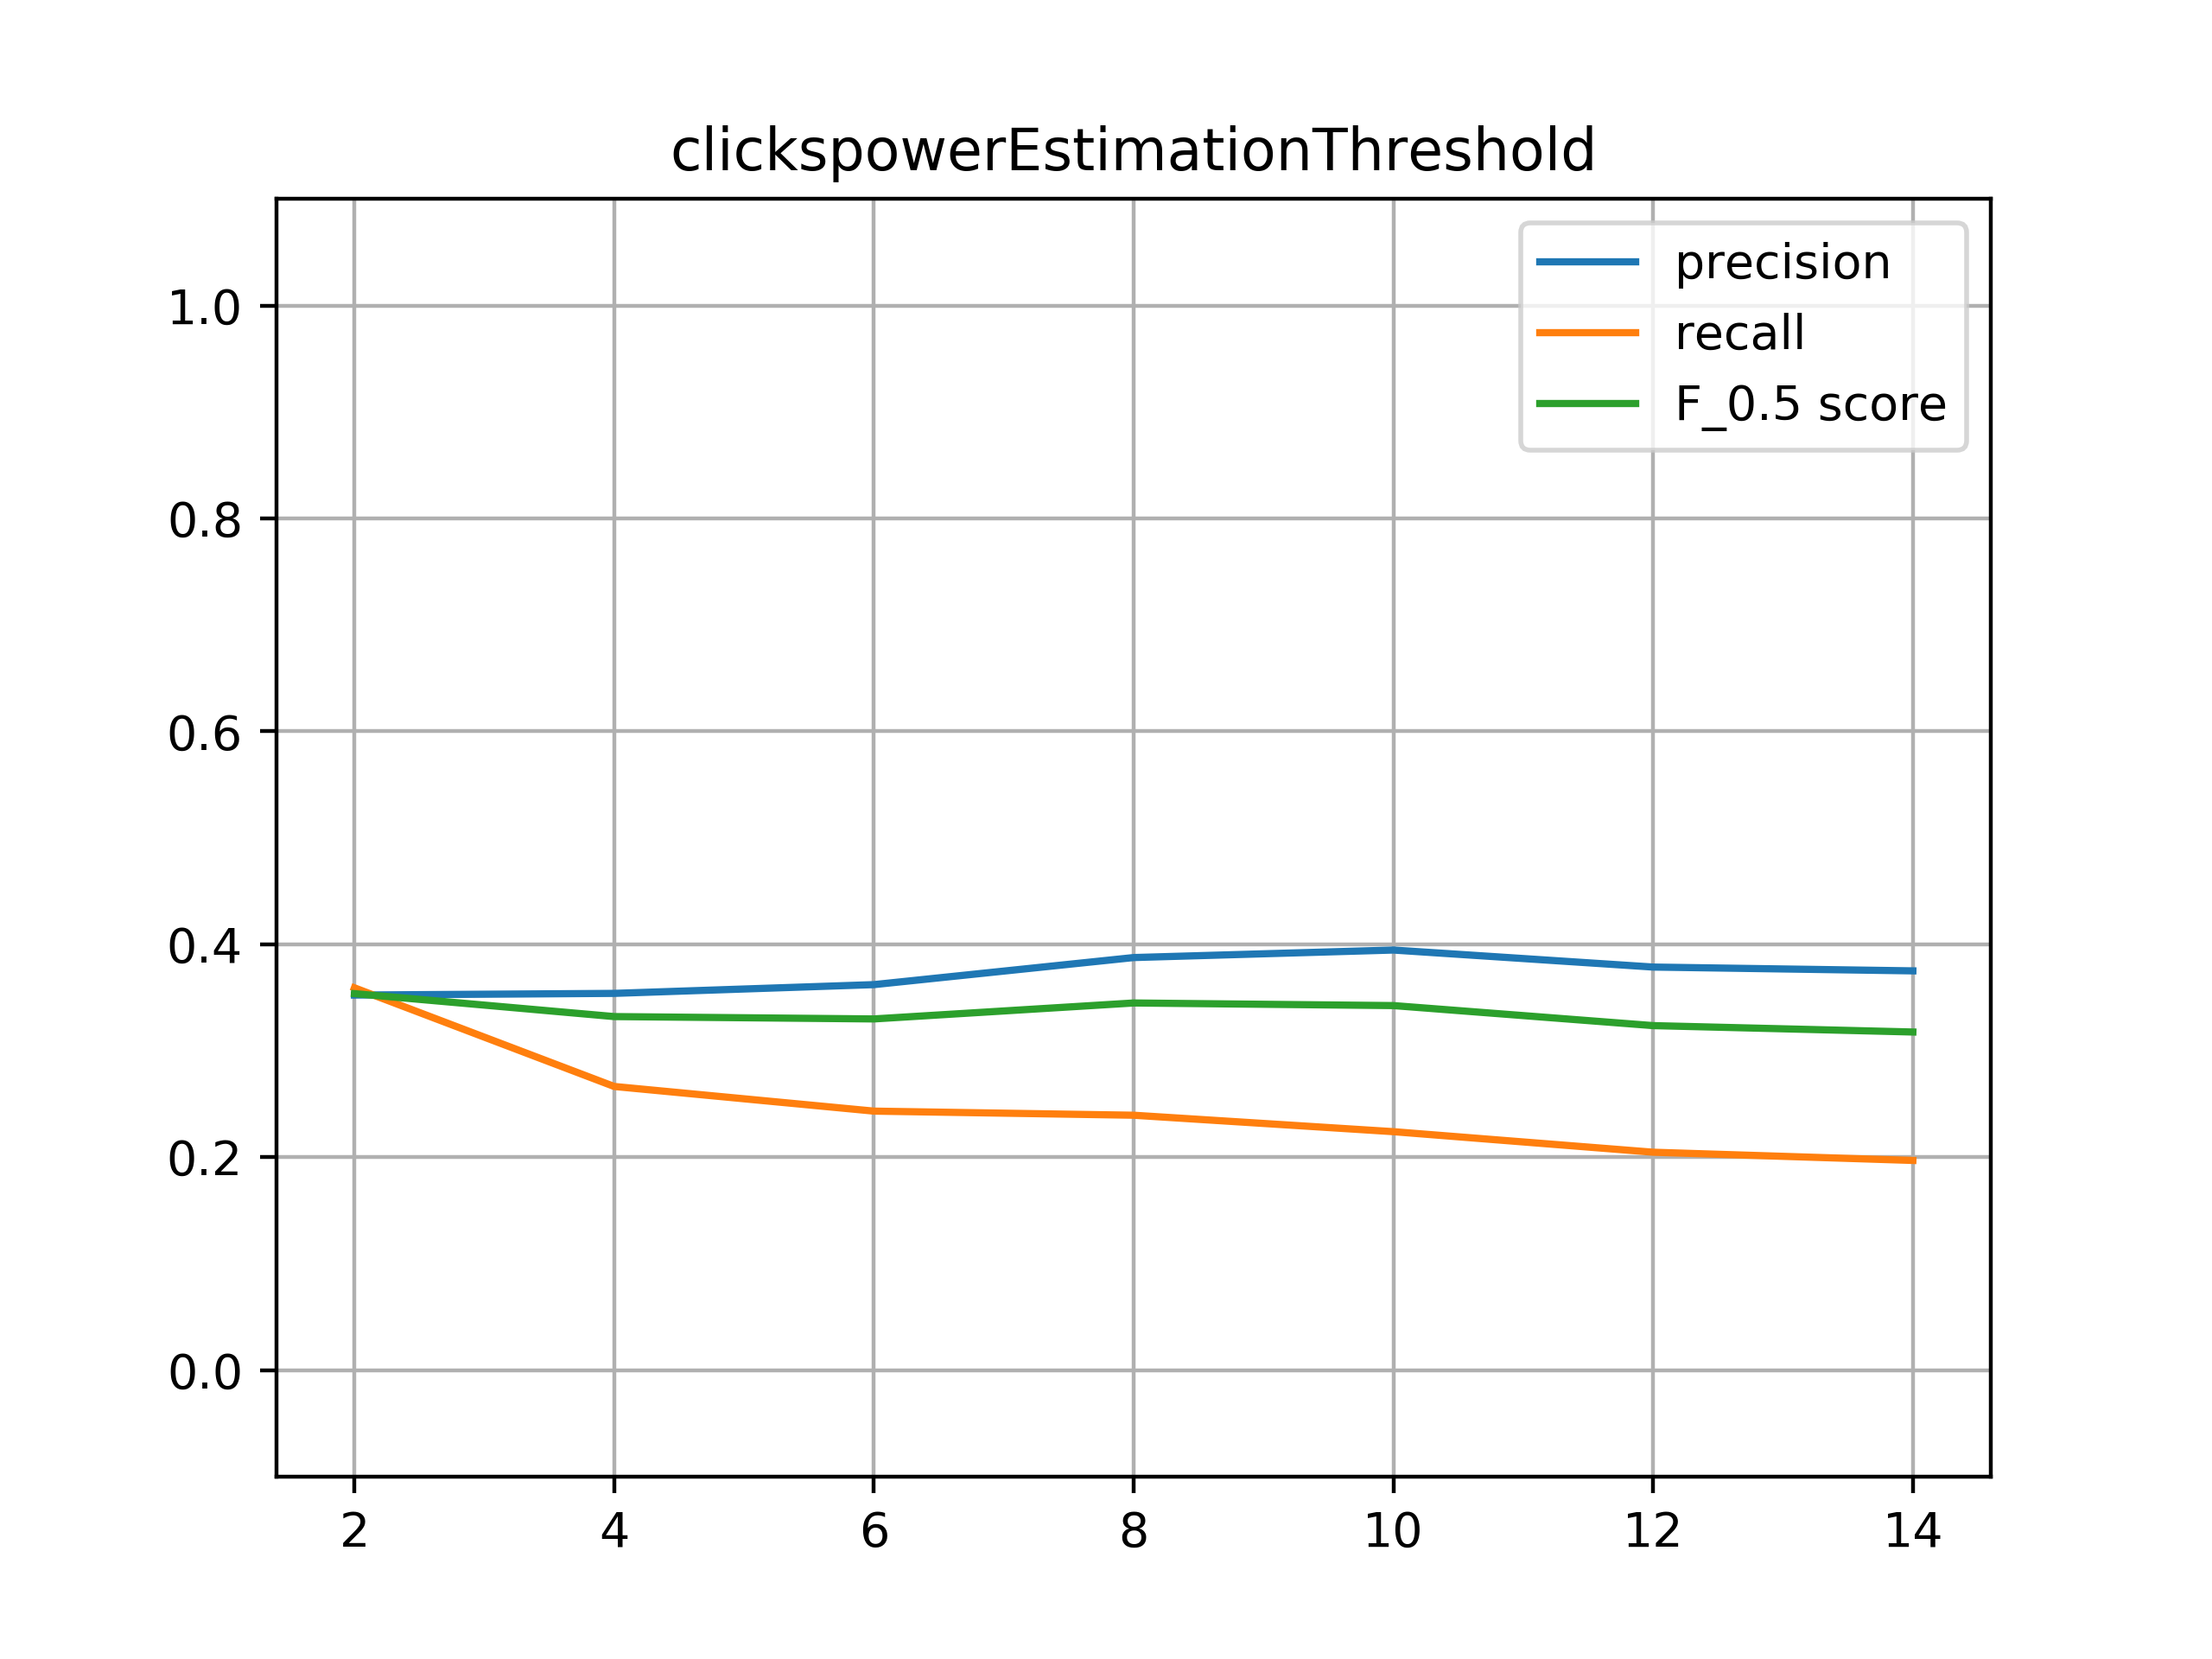
\includegraphics[clip,width=\columnwidth]{Figures/clickspowerEstimationThreshold.png}% 
	\caption{powerEstimationThreshold parameter sweep results (accuracy, F score and recall)}
	\label{fig:clickspowerEstimationThreshold}
\end{figure}

\begin{figure}[!ht]
	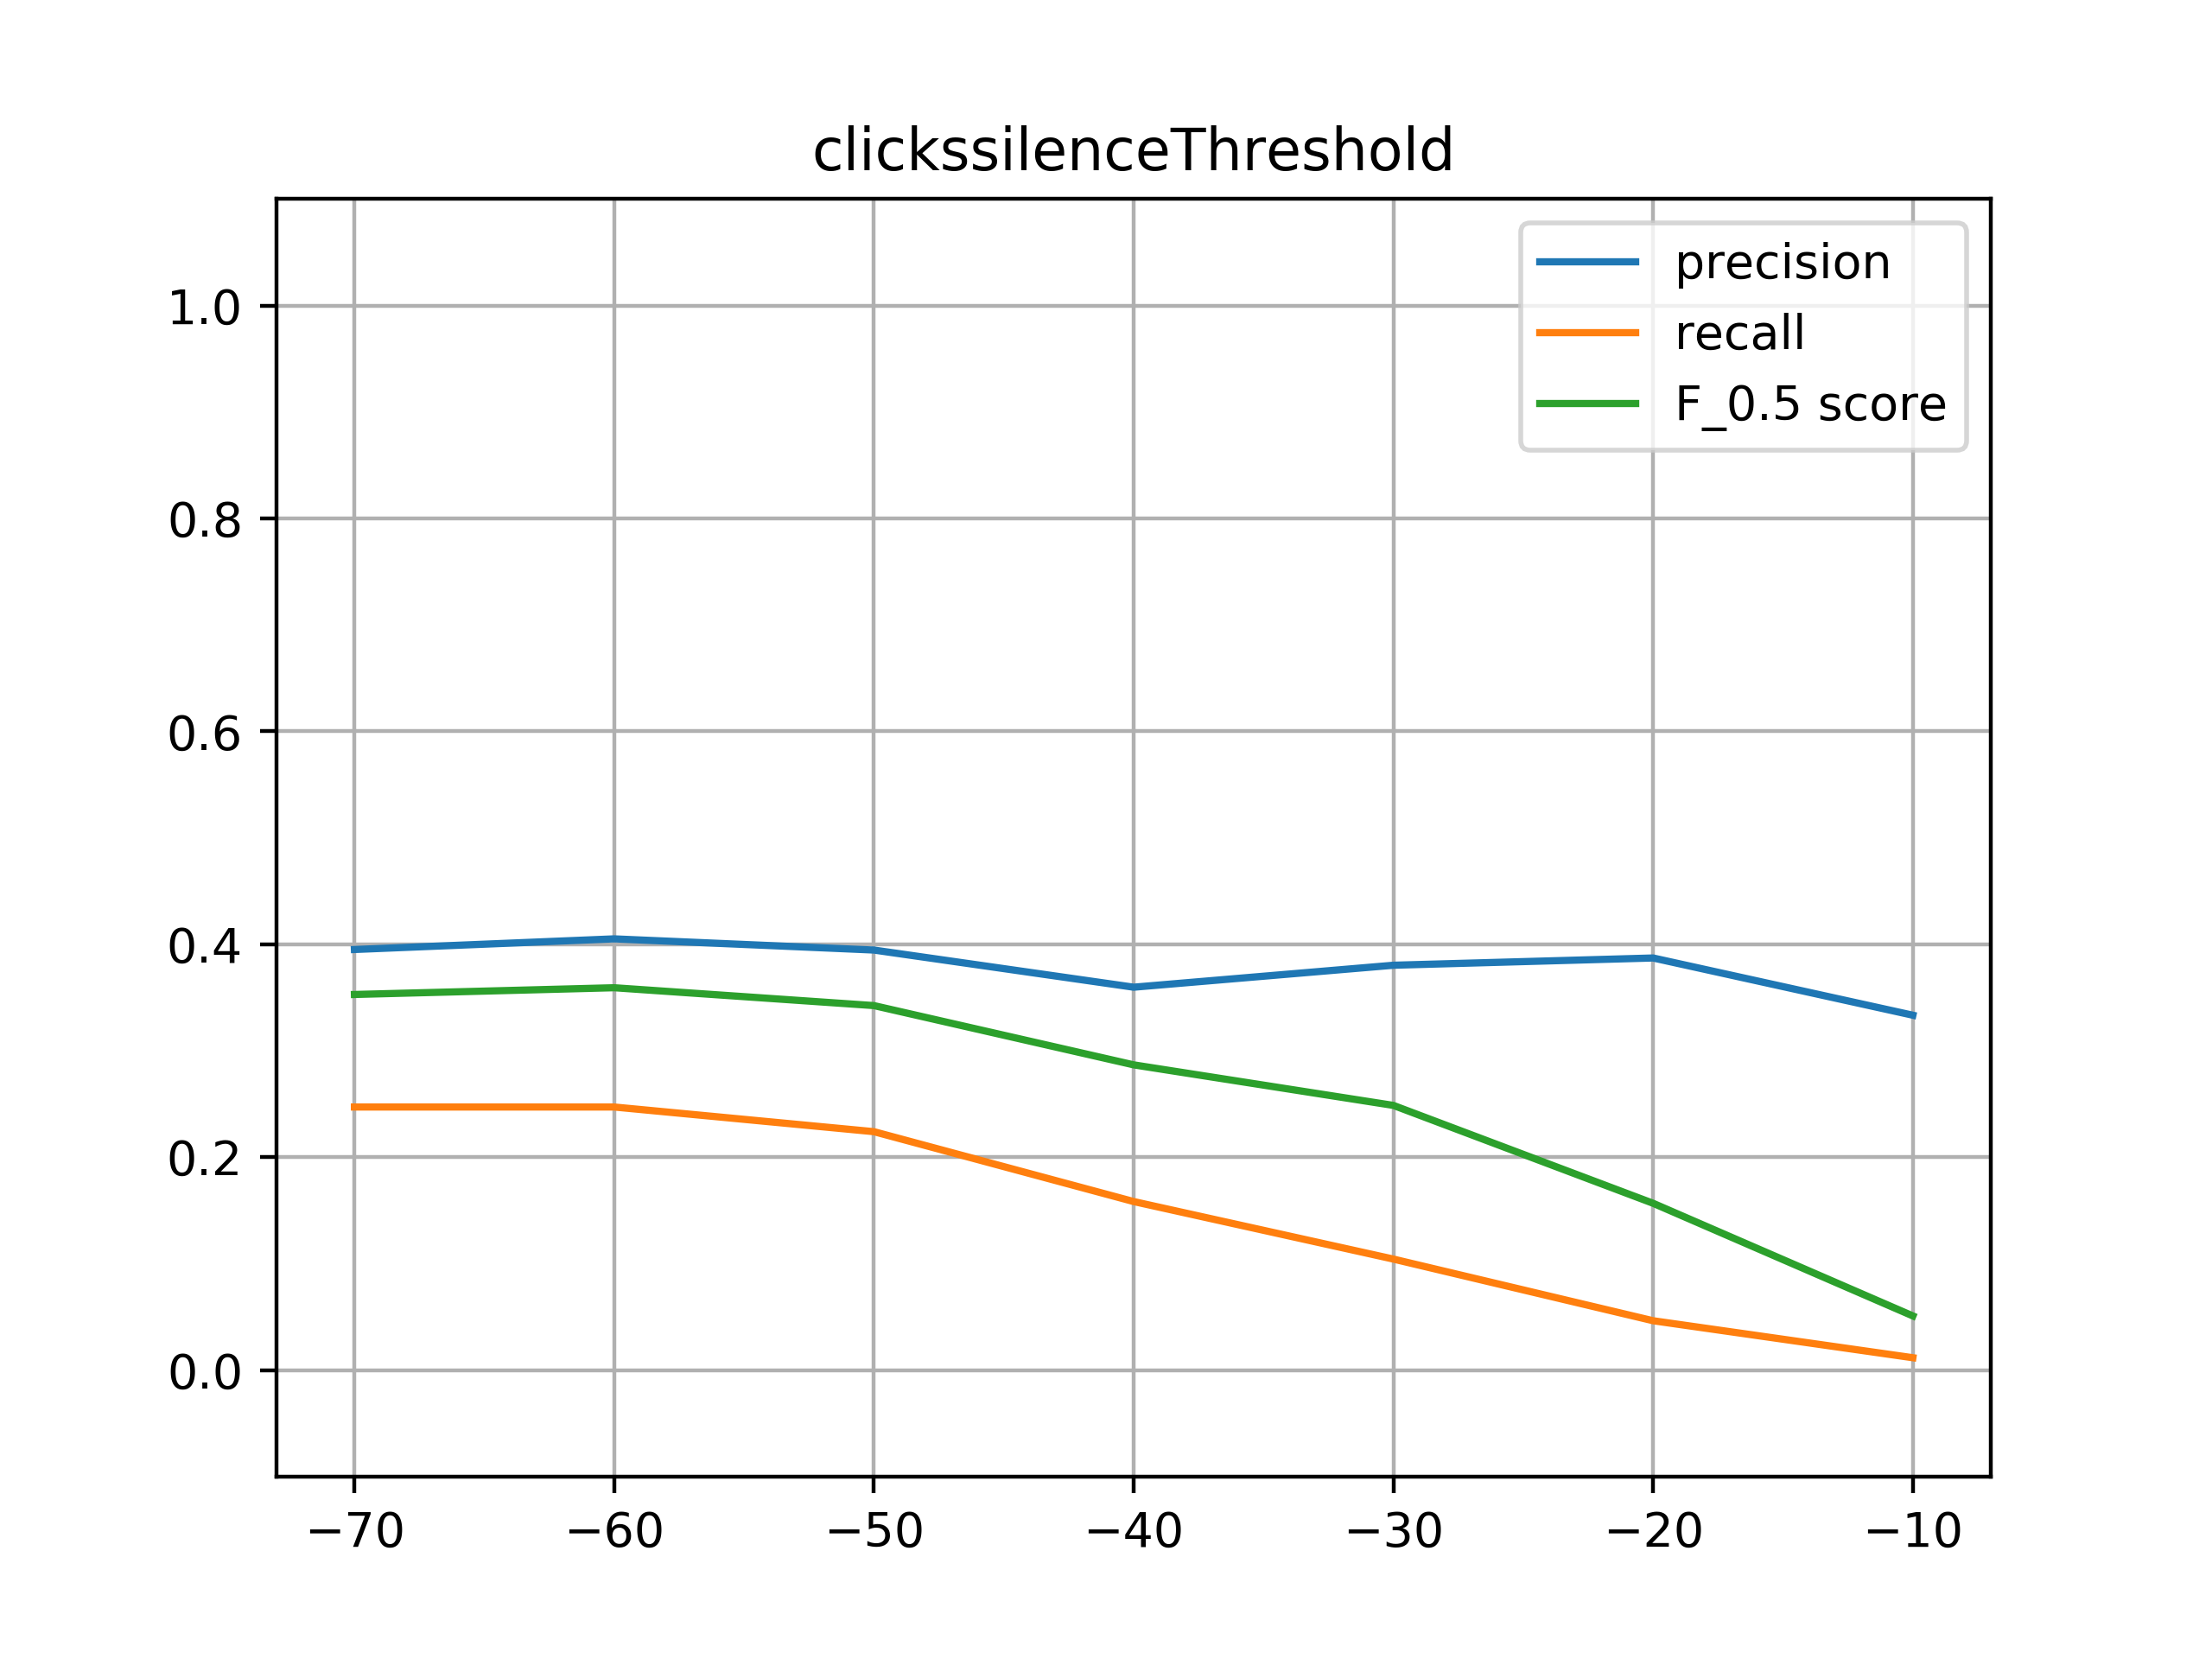
\includegraphics[clip,width=\columnwidth]{Figures/clickssilenceThreshold.png}% 
	\caption{silenceThreshold parameter sweep results (accuracy, F score and recall)}
	\label{fig:clickssilenceThreshold}
\end{figure}

\begin{figure}[!ht]
	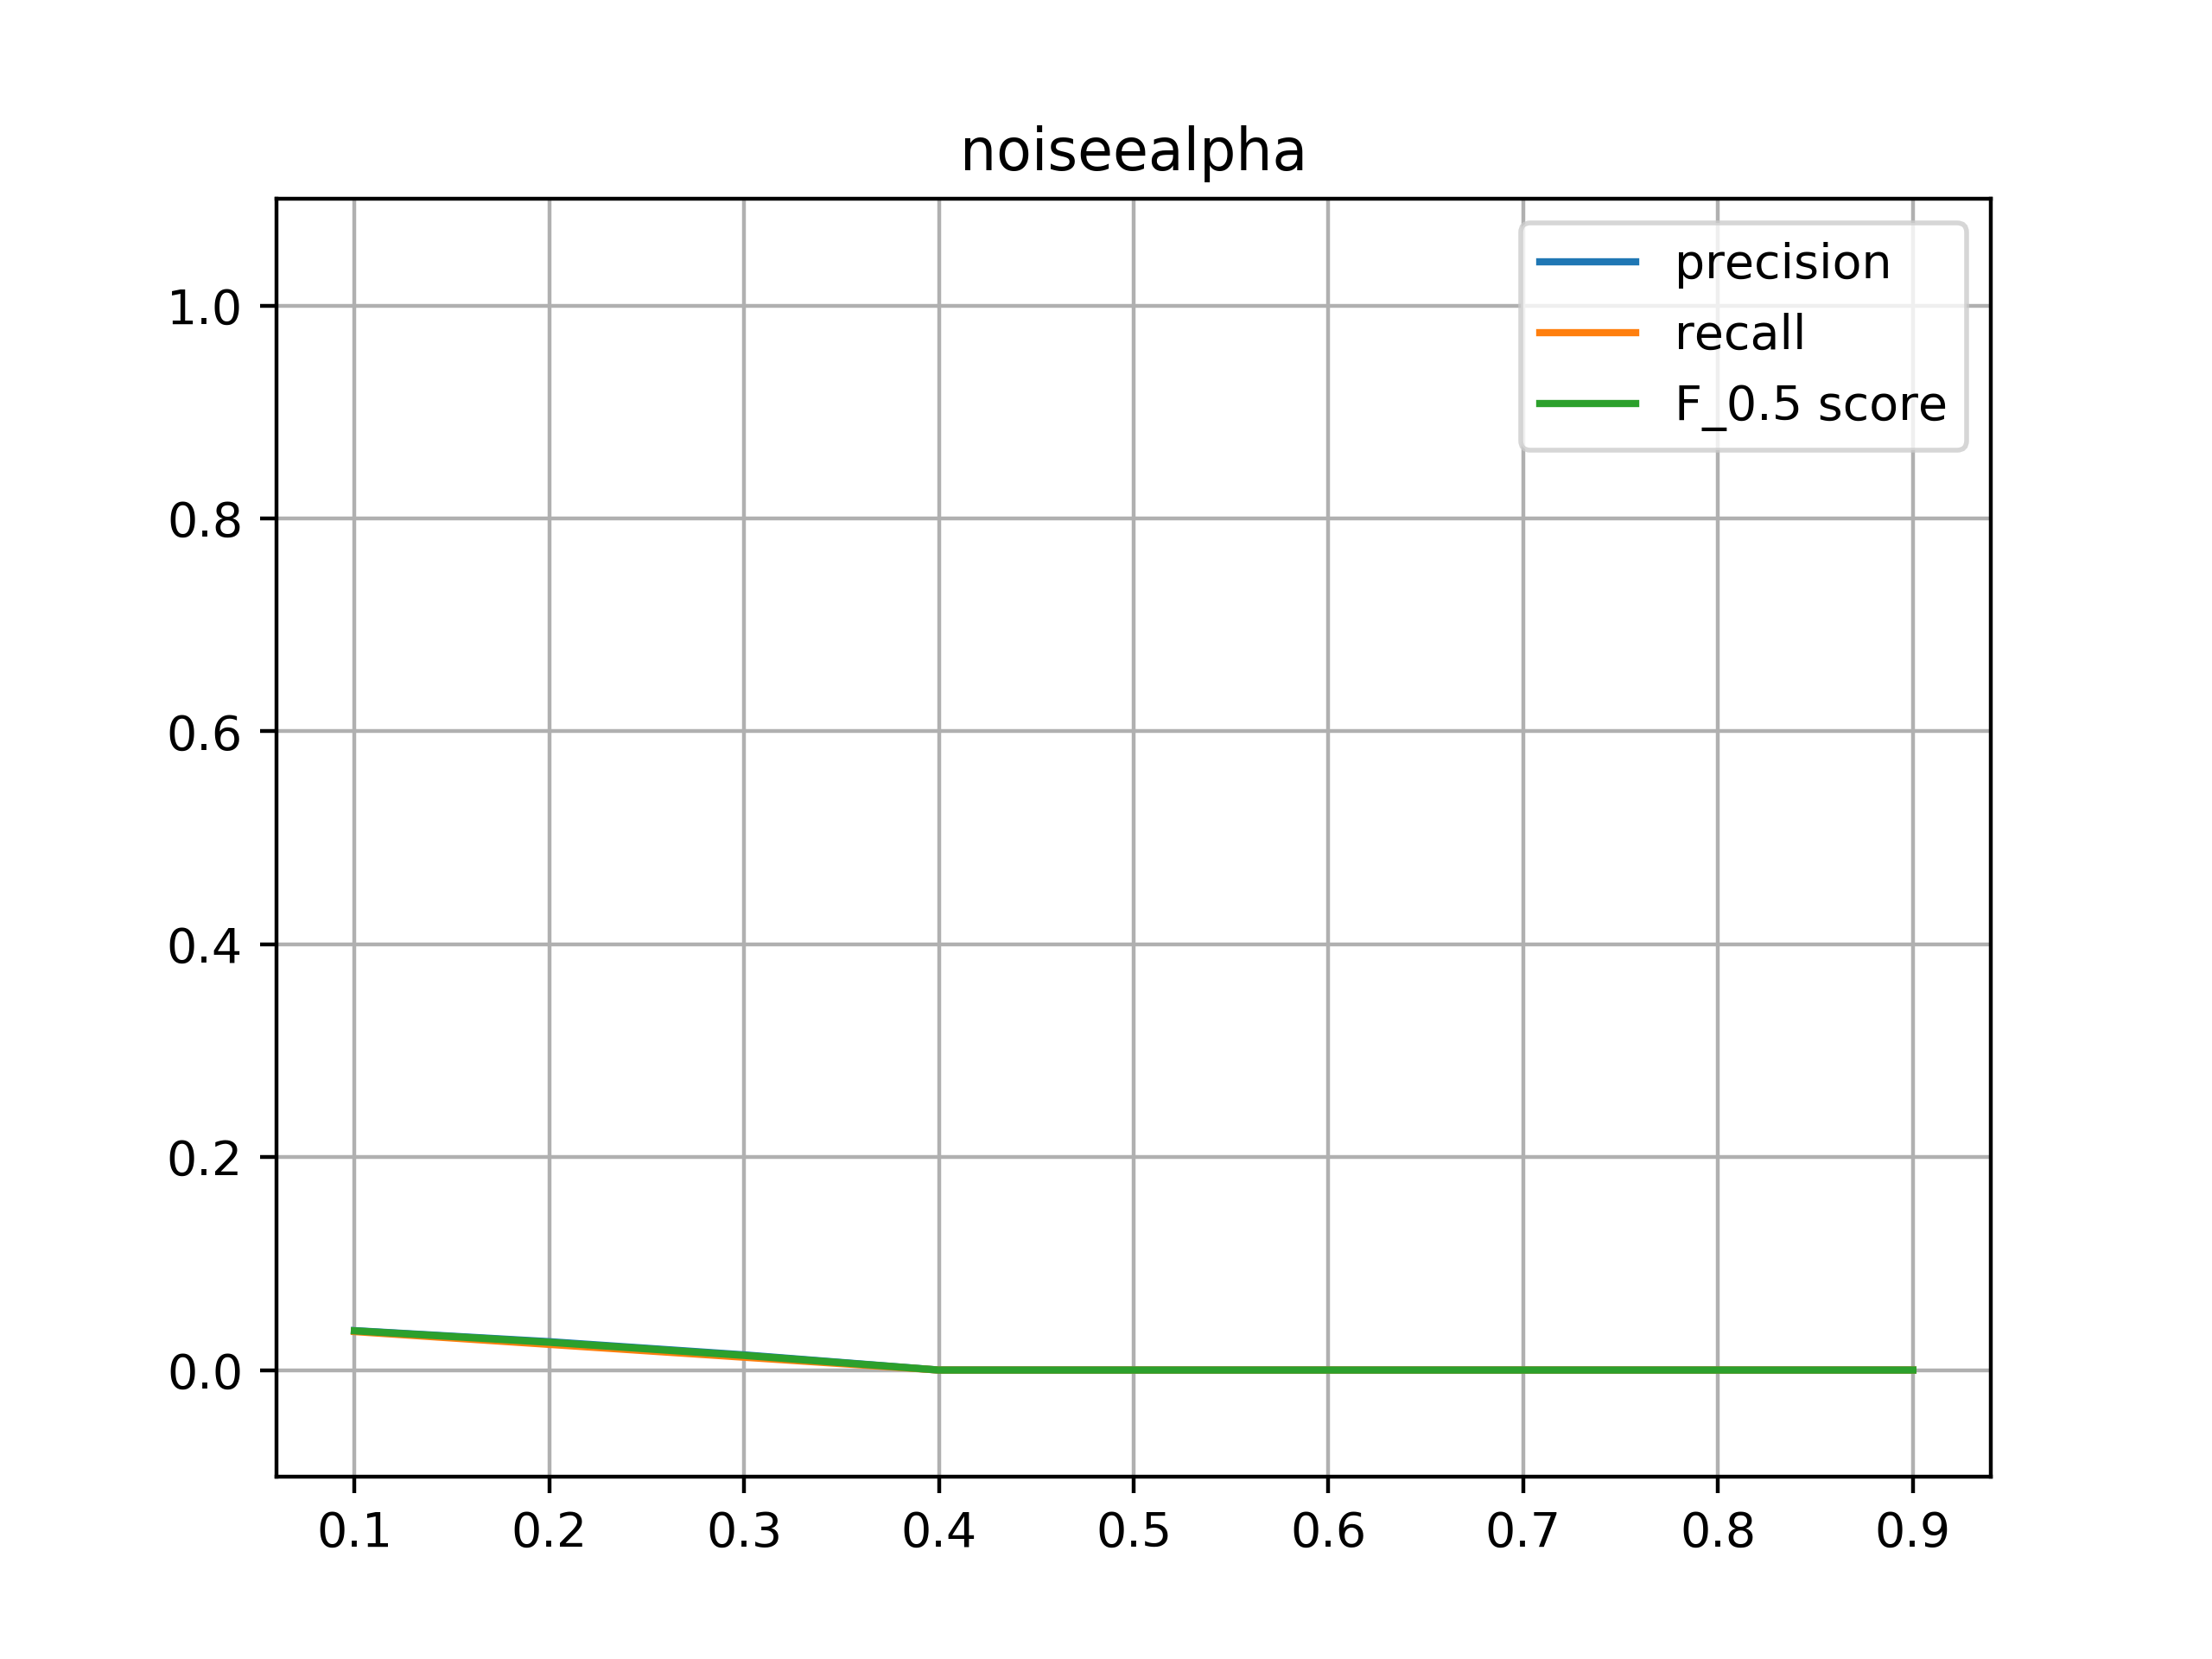
\includegraphics[clip,width=\columnwidth]{Figures/noiseealpha.png}% 
	\caption{alpha parameter sweep results (accuracy, F score and recall)}
	\label{fig:noiseealpha}
\end{figure}

\begin{figure}[!ht]
	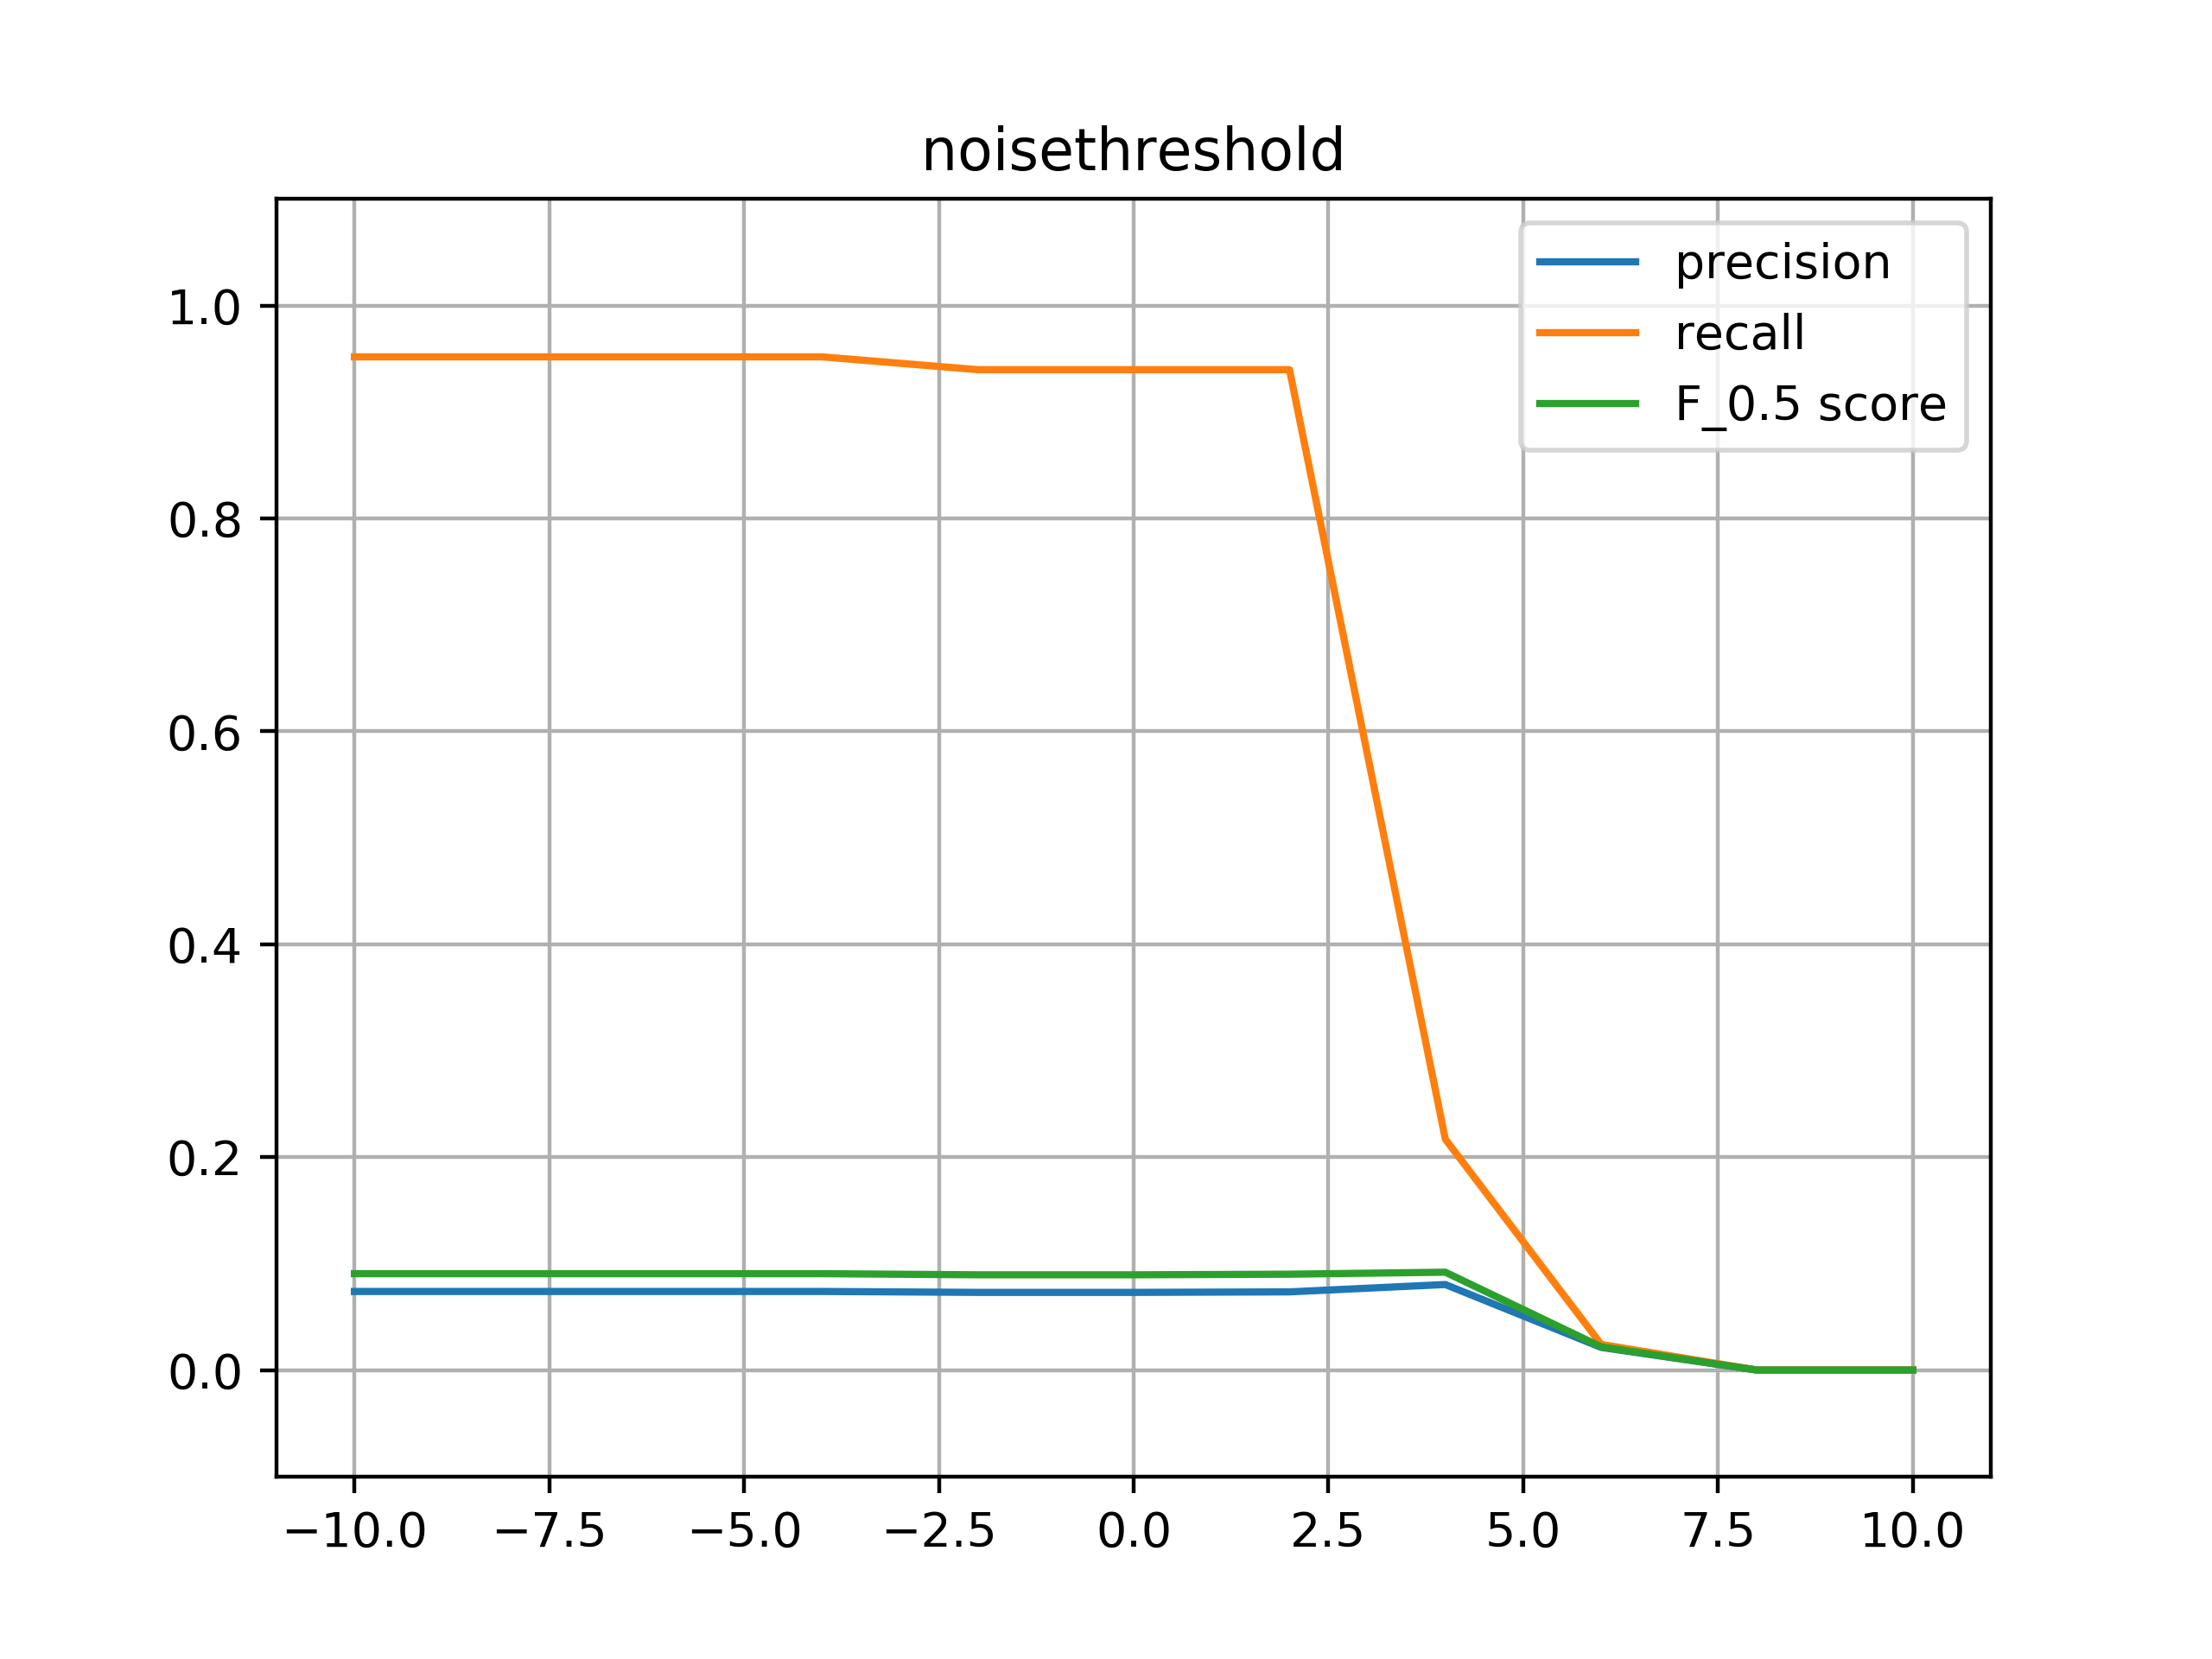
\includegraphics[clip,width=\columnwidth]{Figures/noisethreshold.png}% 
	\caption{threshold parameter sweep results (accuracy, F score and recall)}
	\label{fig:noisethreshold}
\end{figure}

\begin{figure}[!ht]
	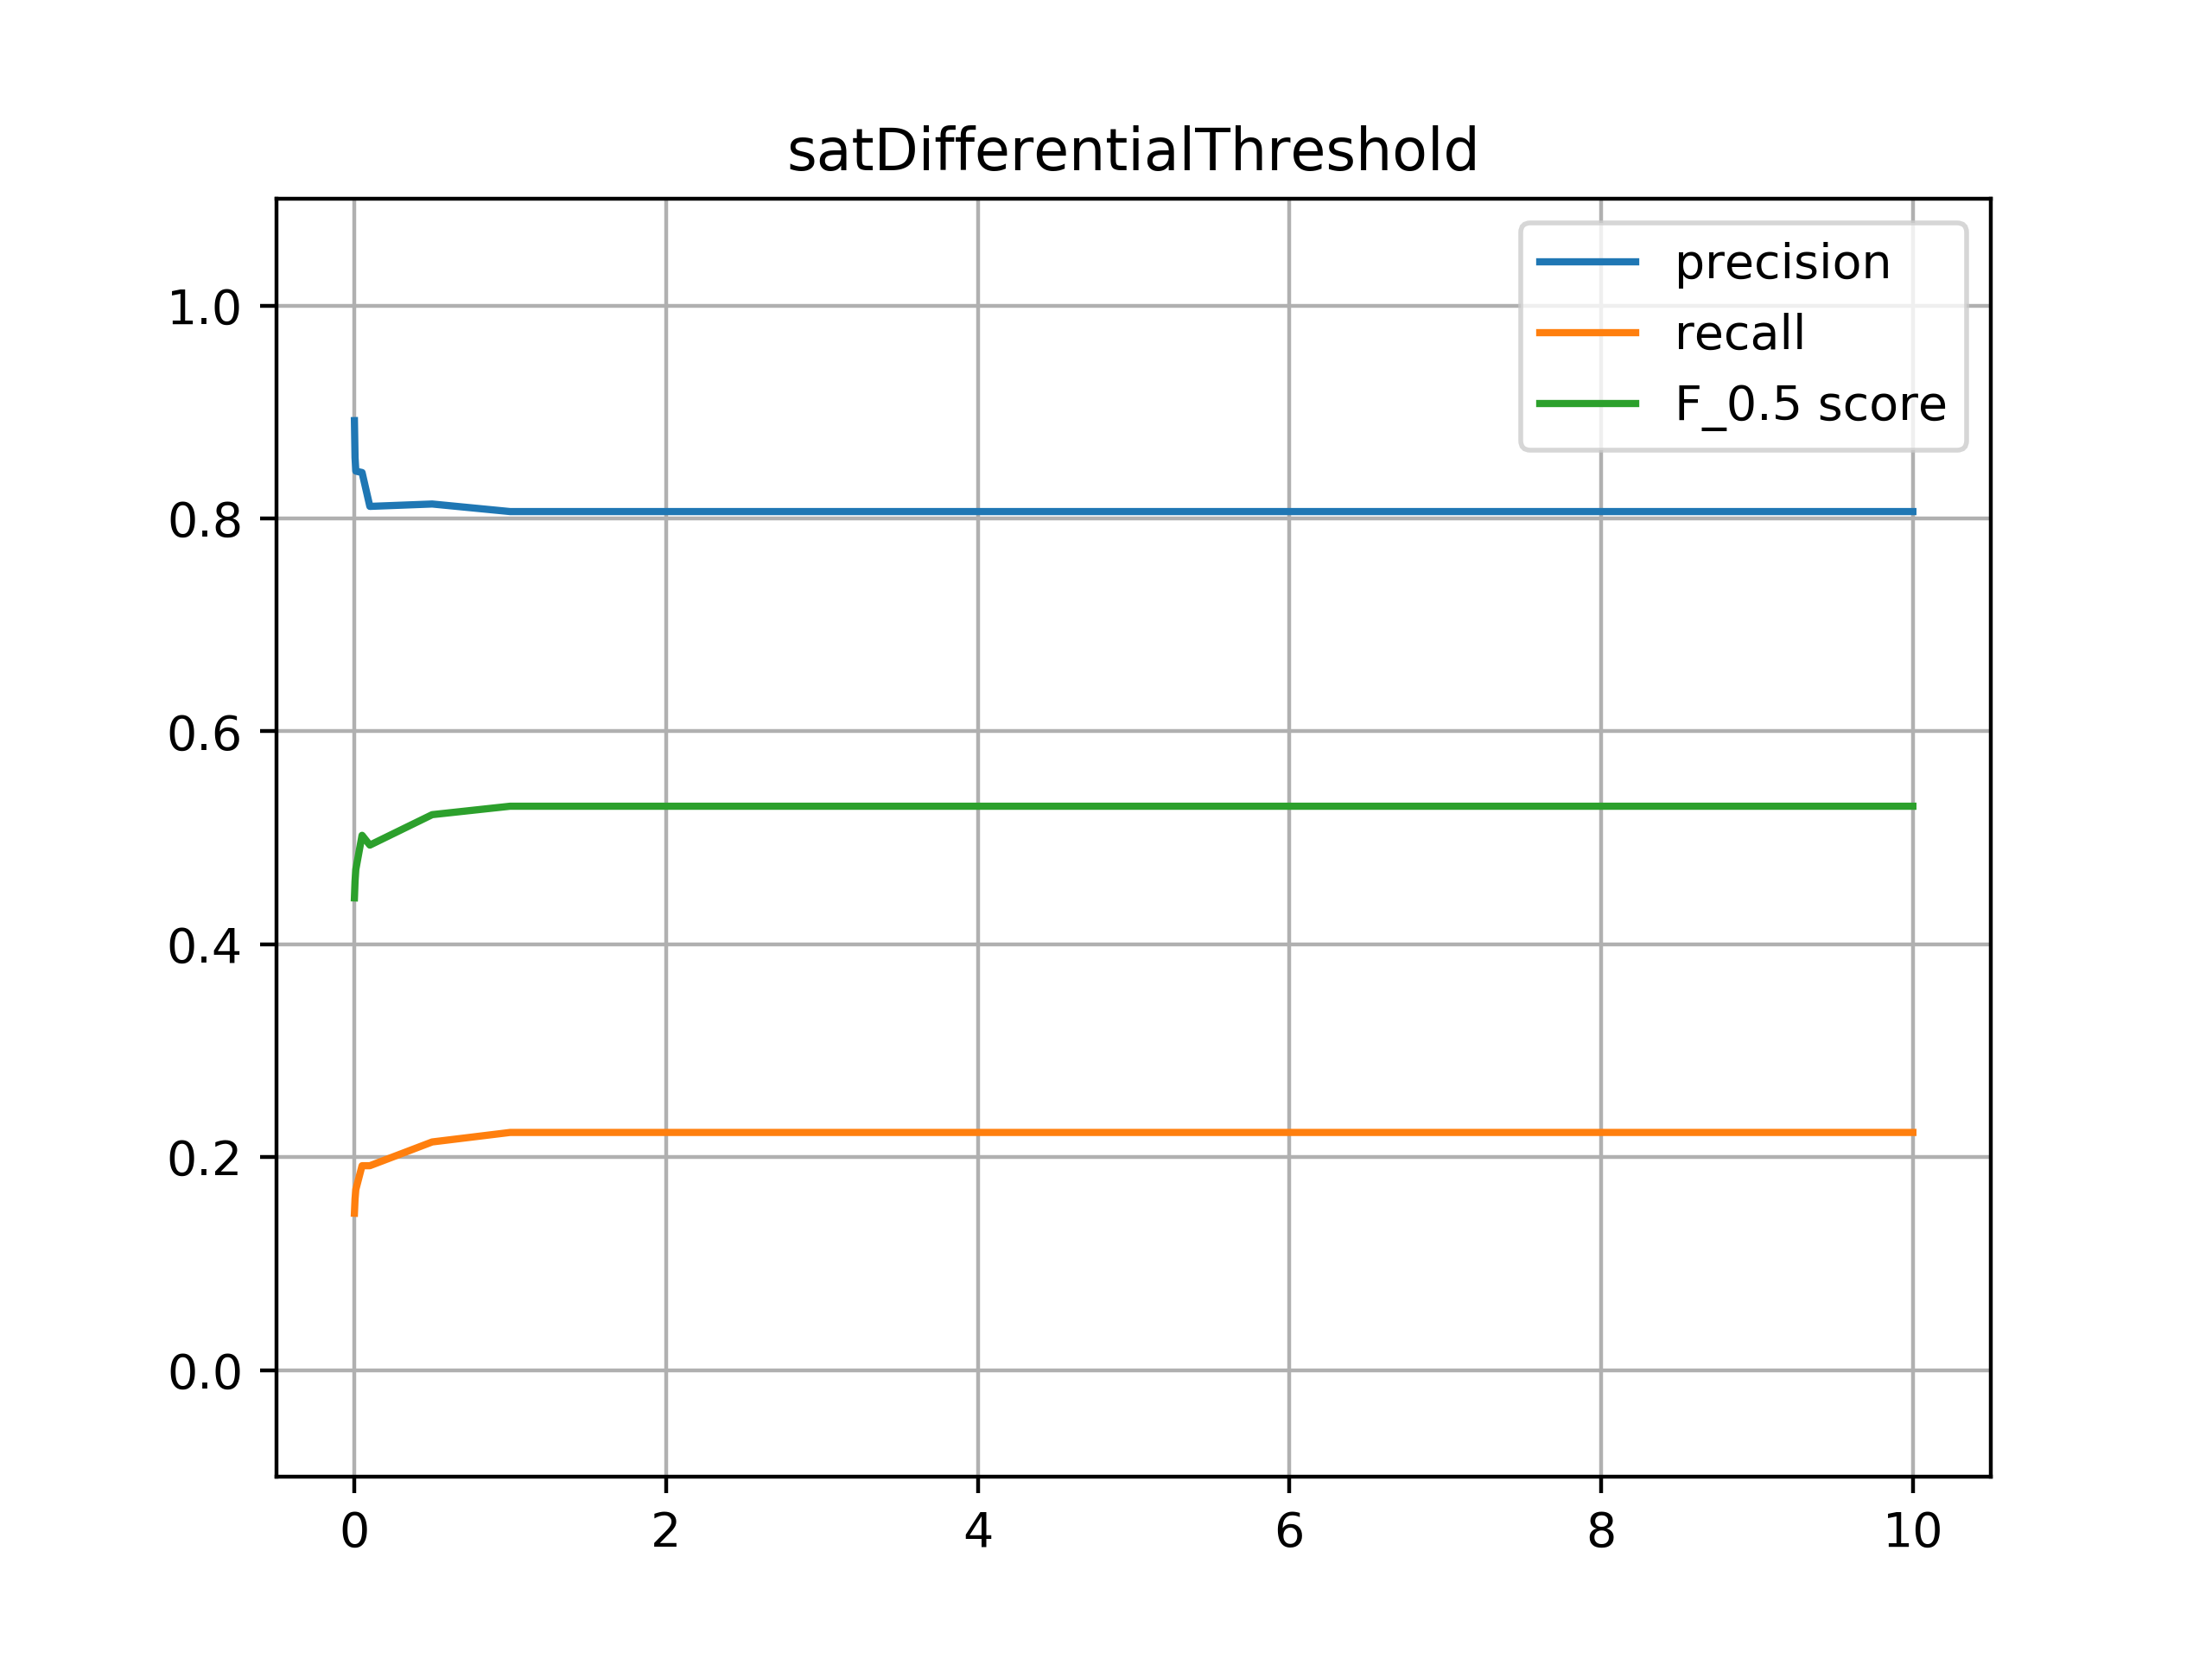
\includegraphics[clip,width=\columnwidth]{Figures/satDifferentialThreshold.png}% 
	\caption{differentialThreshold parameter sweep results (accuracy, F score and recall)}
	\label{fig:satDifferentialThreshold}
\end{figure}

\begin{figure}[!ht]
	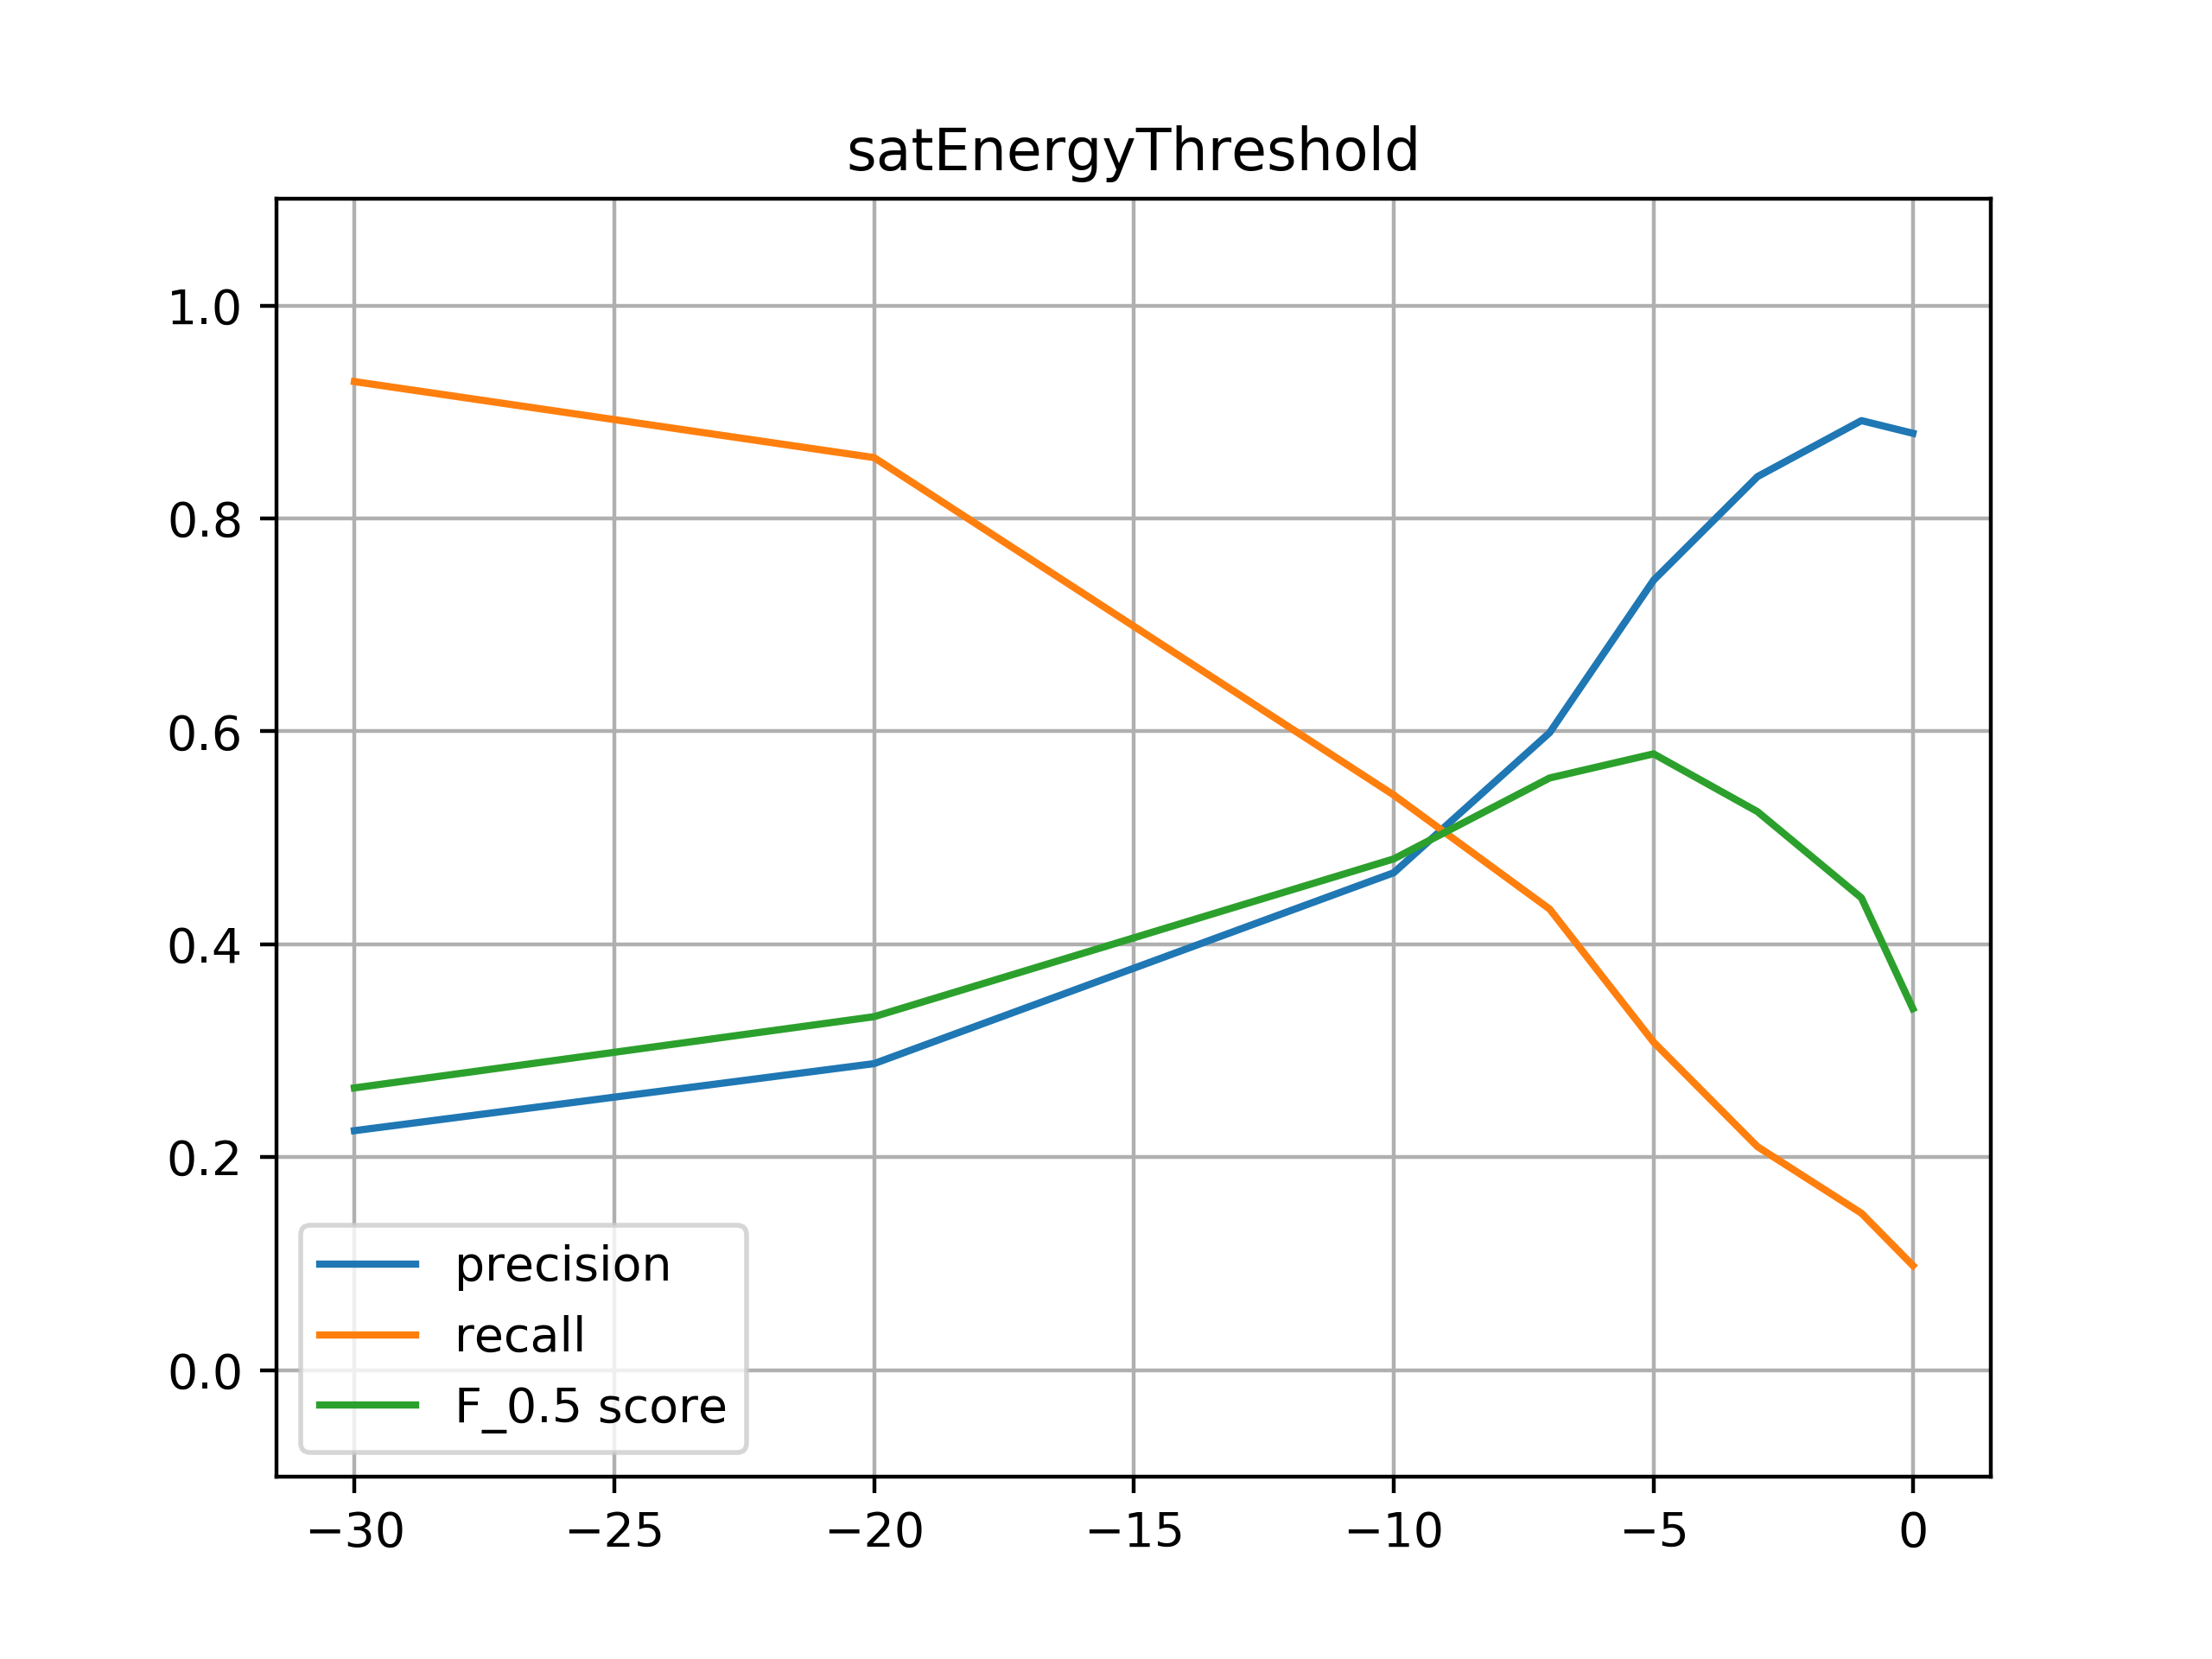
\includegraphics[clip,width=\columnwidth]{Figures/satEnergyThreshold.png}% 
	\caption{energyThreshold parameter sweep results (accuracy, F score and recall)}
	\label{fig:satEnergyThreshold}
\end{figure}

\begin{figure}[!ht]
	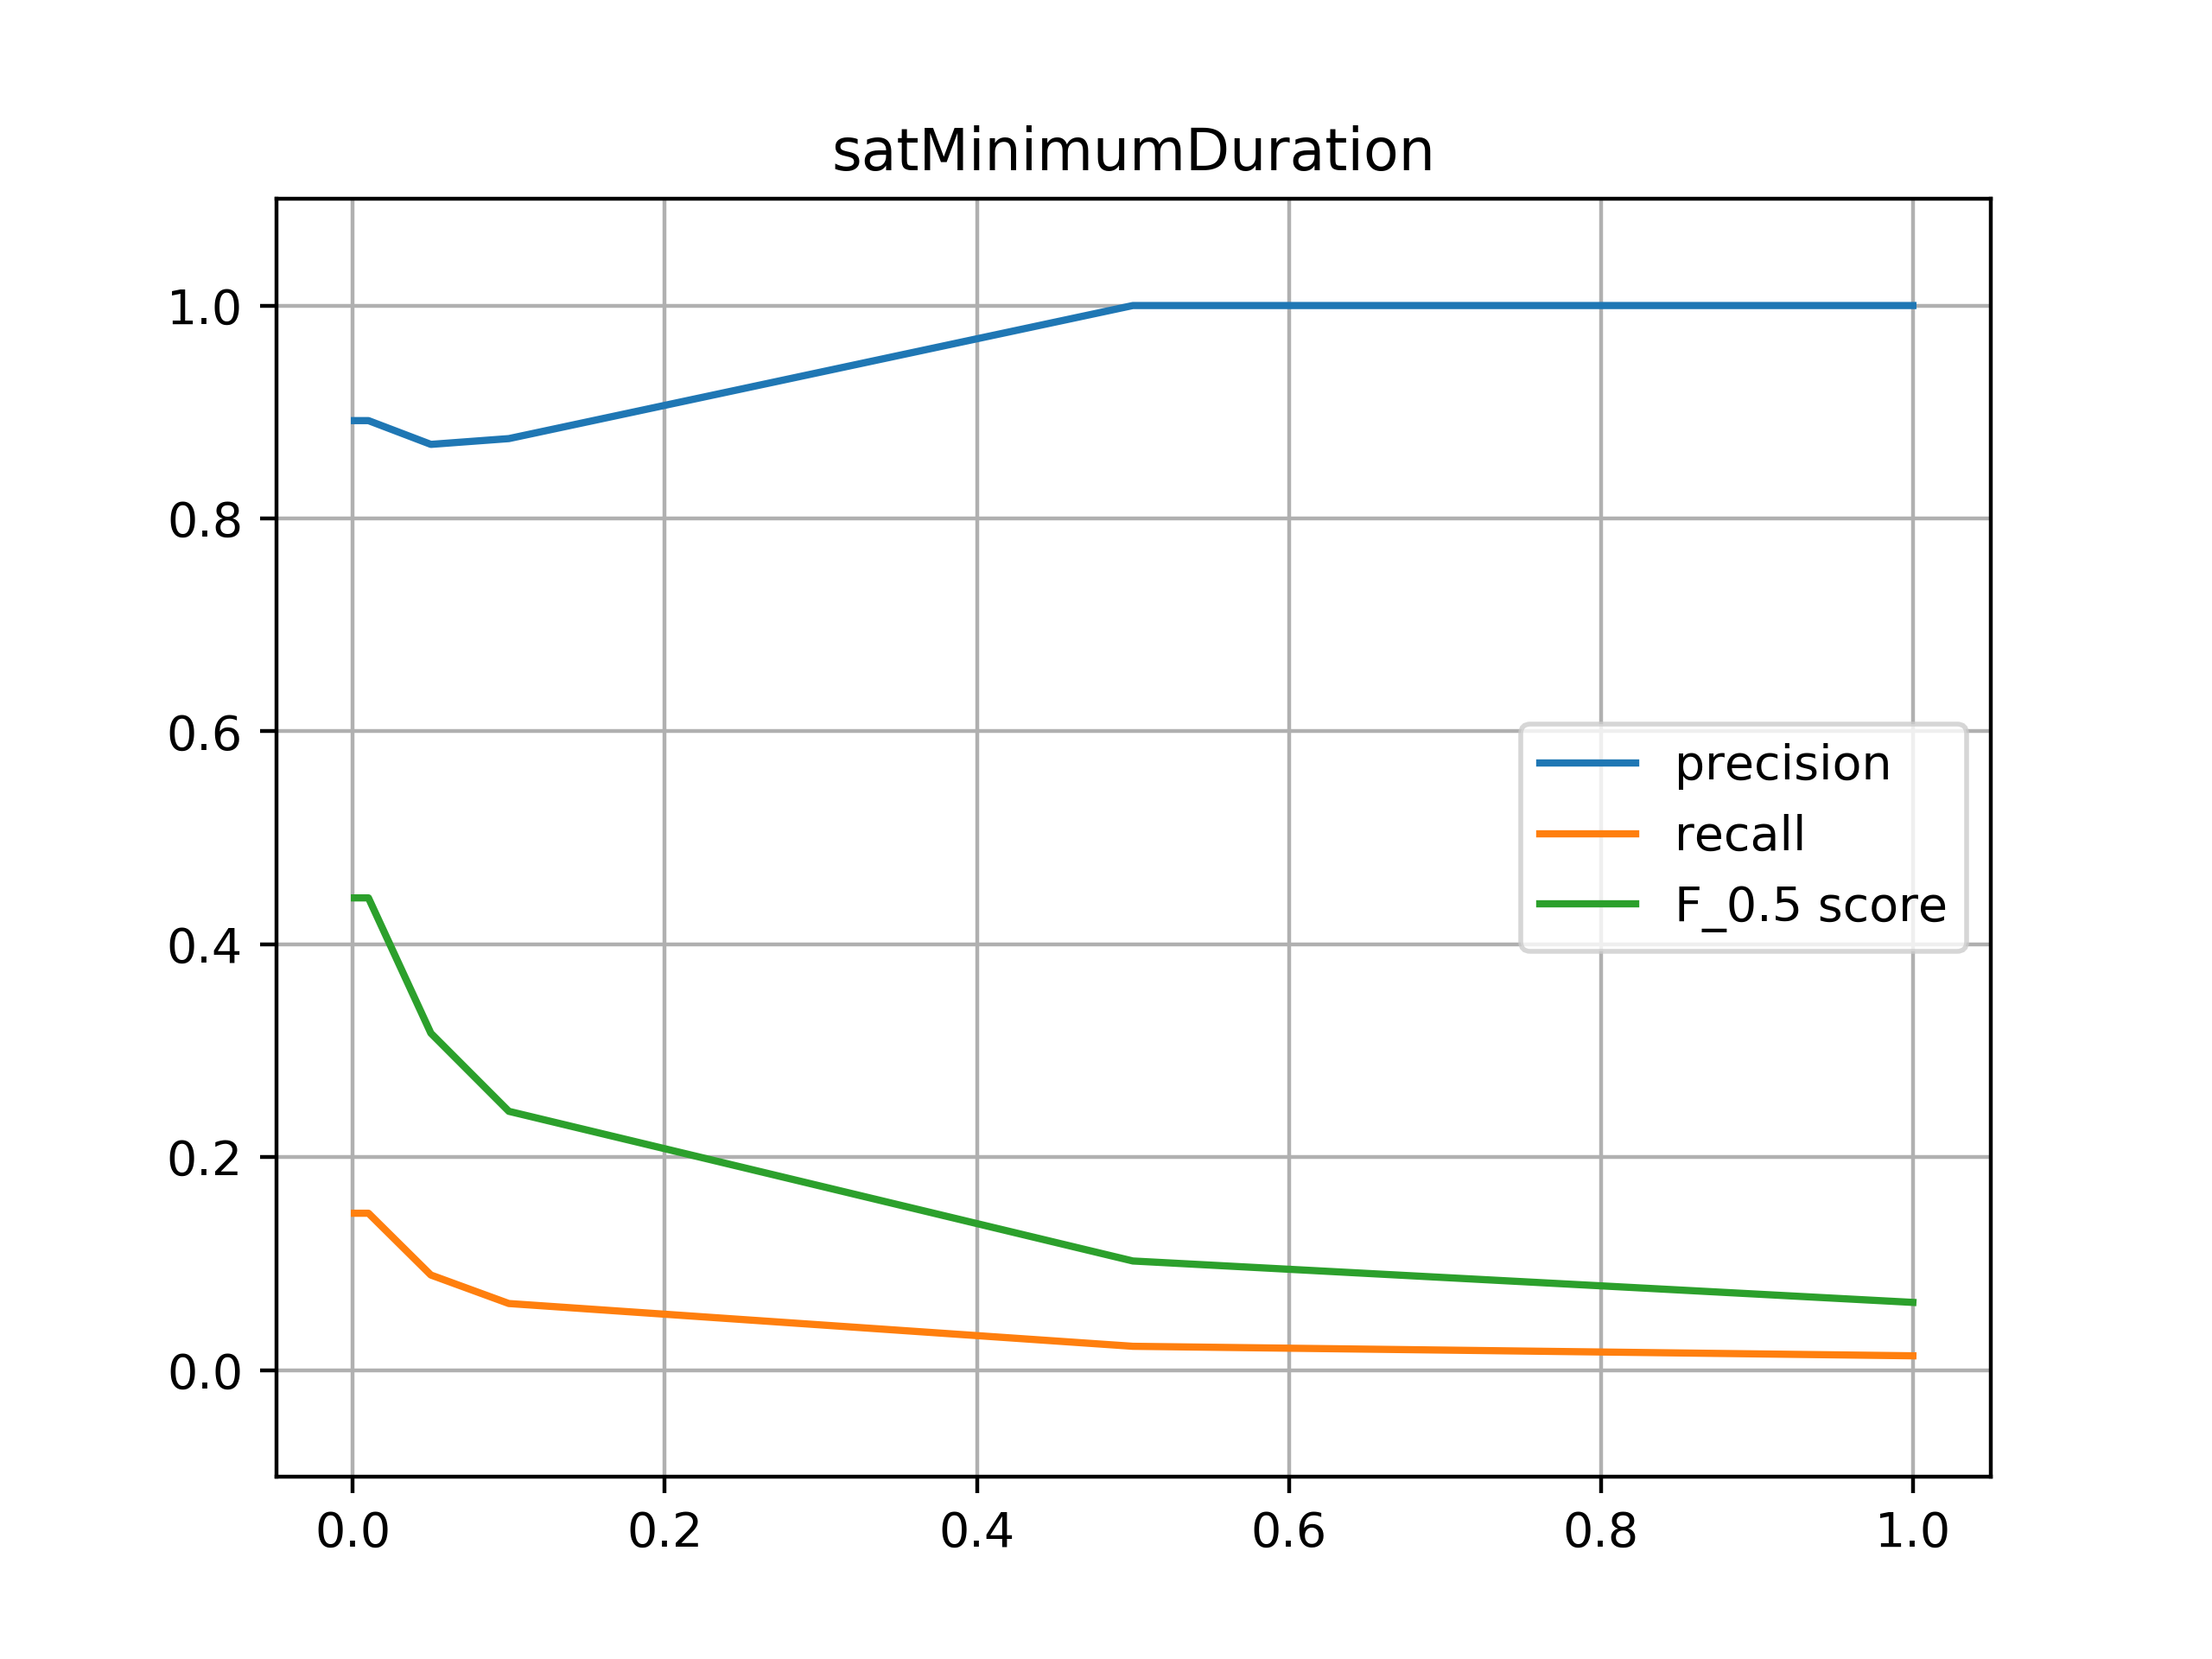
\includegraphics[clip,width=\columnwidth]{Figures/satMinimumDuration.png}% 
	\caption{minimumDuration parameter sweep results (accuracy, F score and recall)}
	\label{fig:satMinimumDuration}
\end{figure}

\begin{figure}[!ht]
	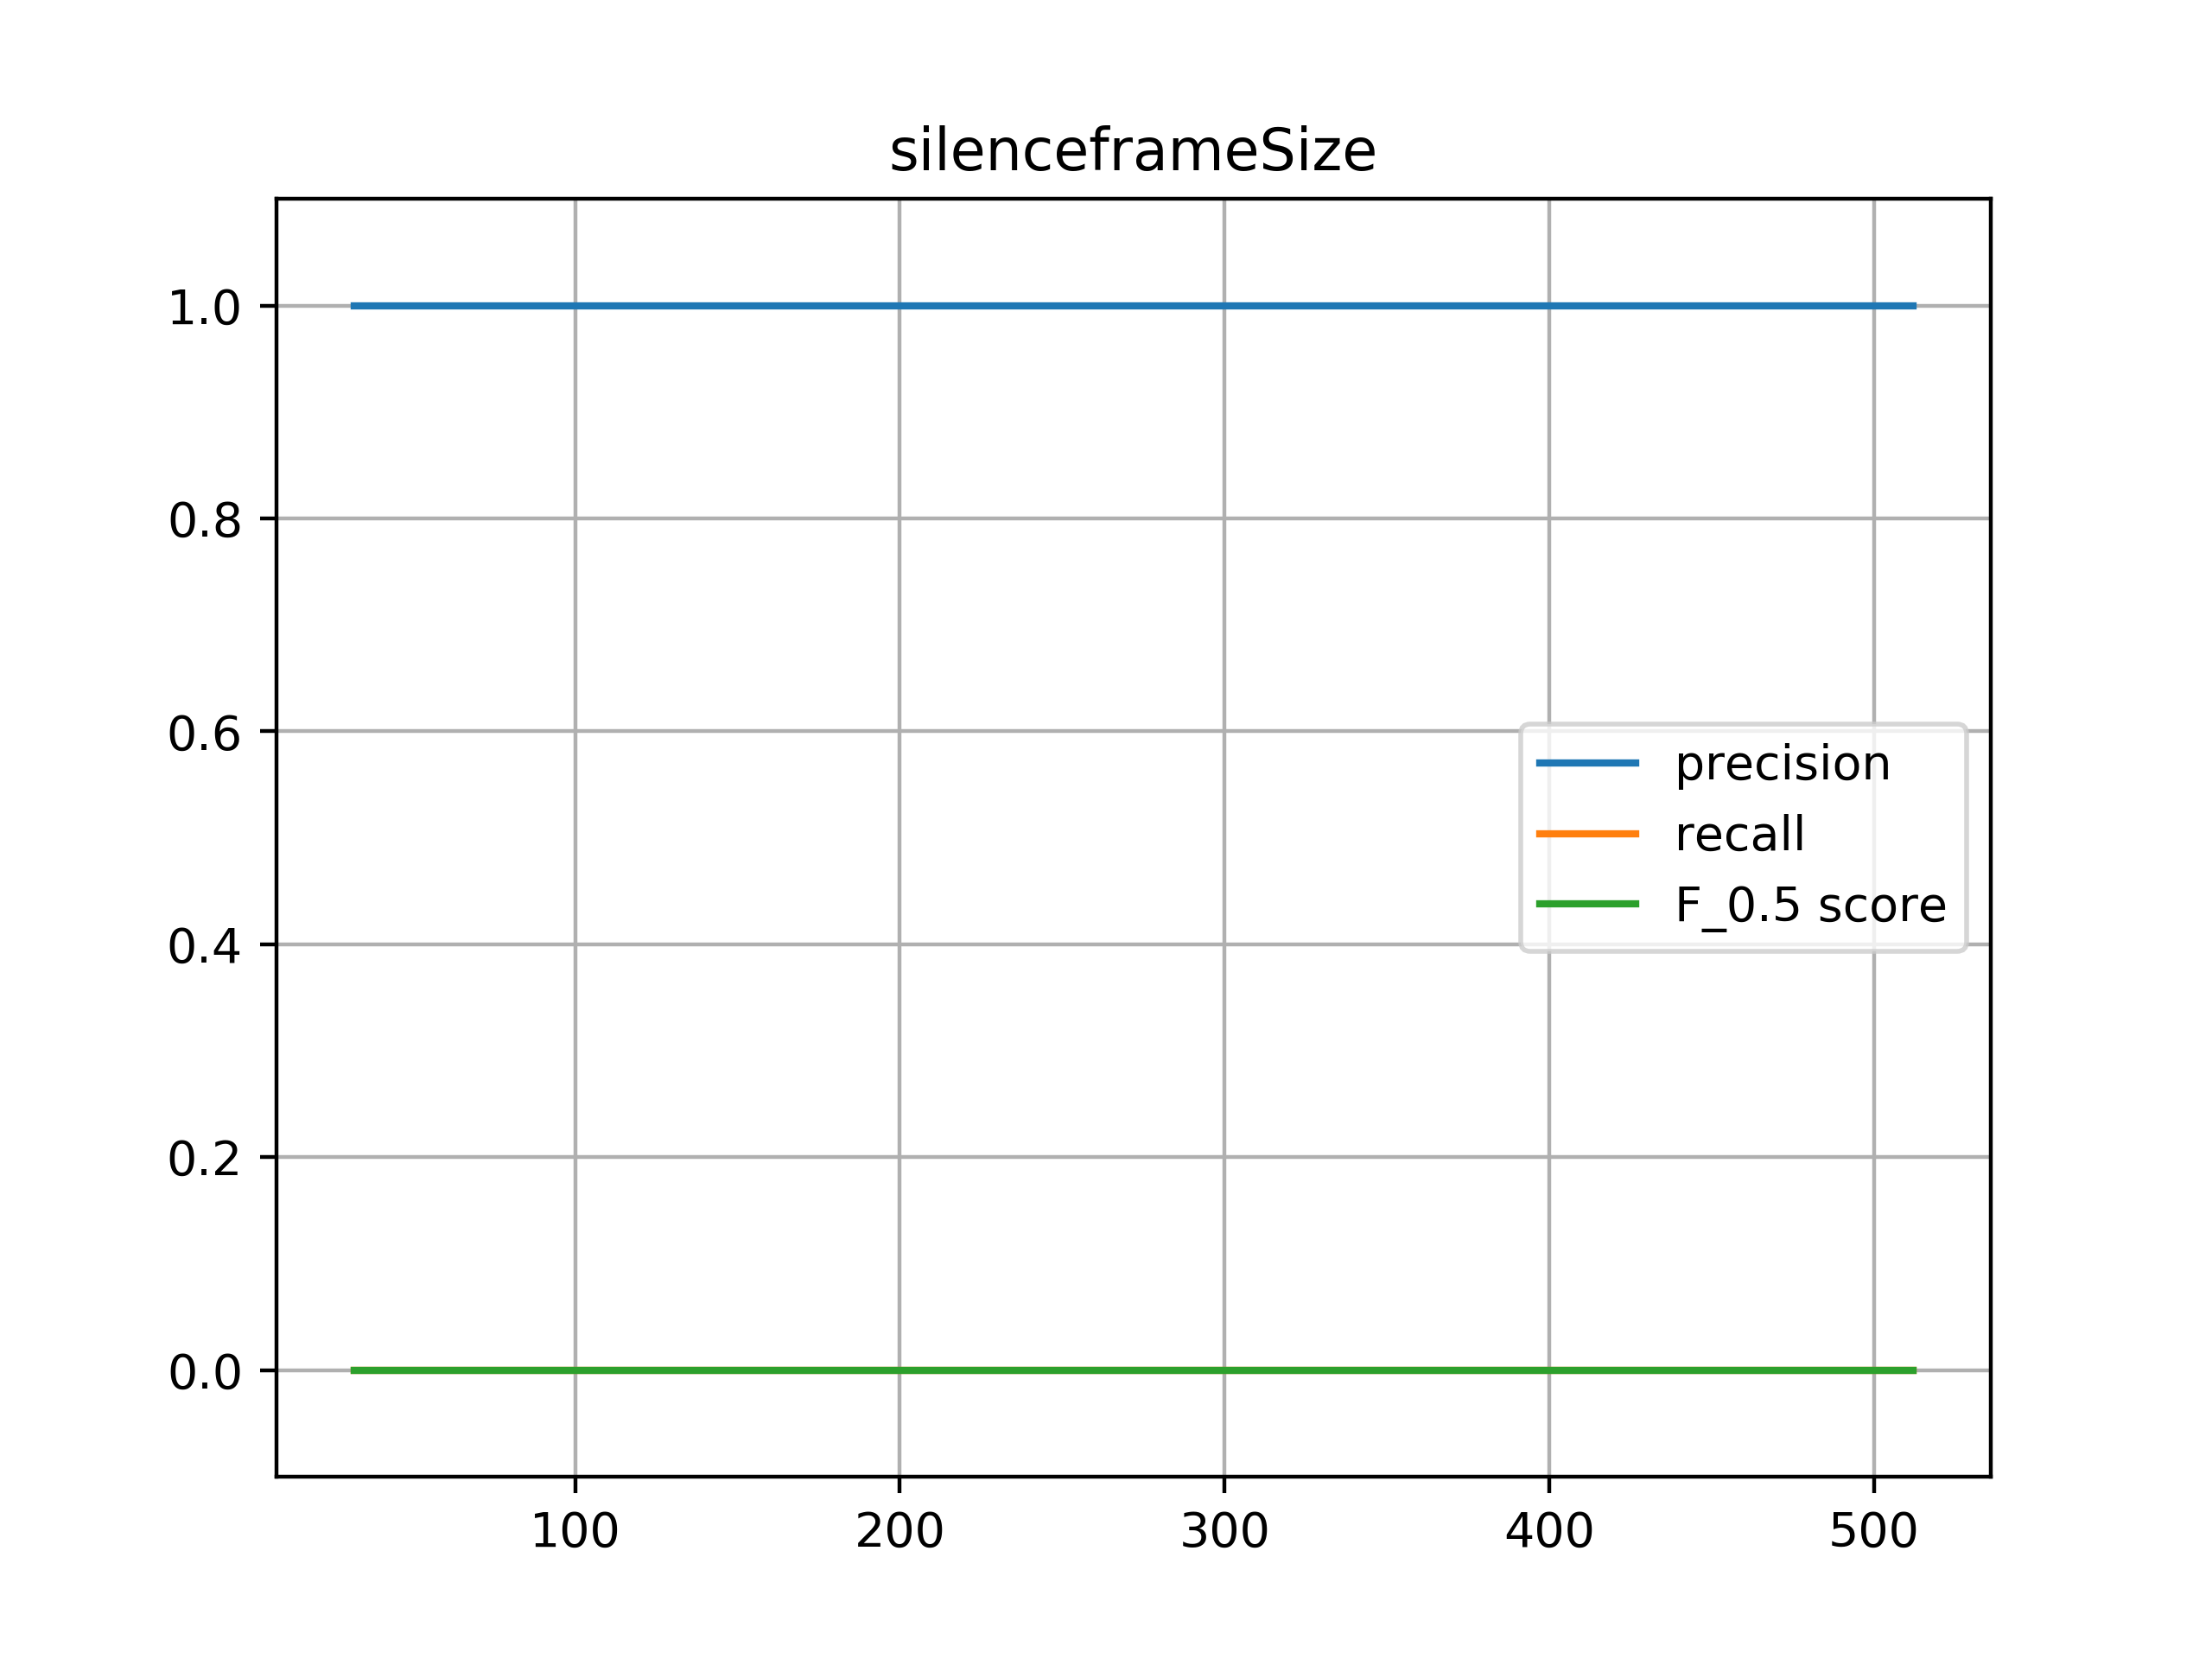
\includegraphics[clip,width=\columnwidth]{Figures/silenceframeSize.png}% 
	\caption{frameSize parameter sweep results (accuracy, F score and recall)}
	\label{fig:silenceframeSize}
\end{figure}

\begin{figure}[!ht]
	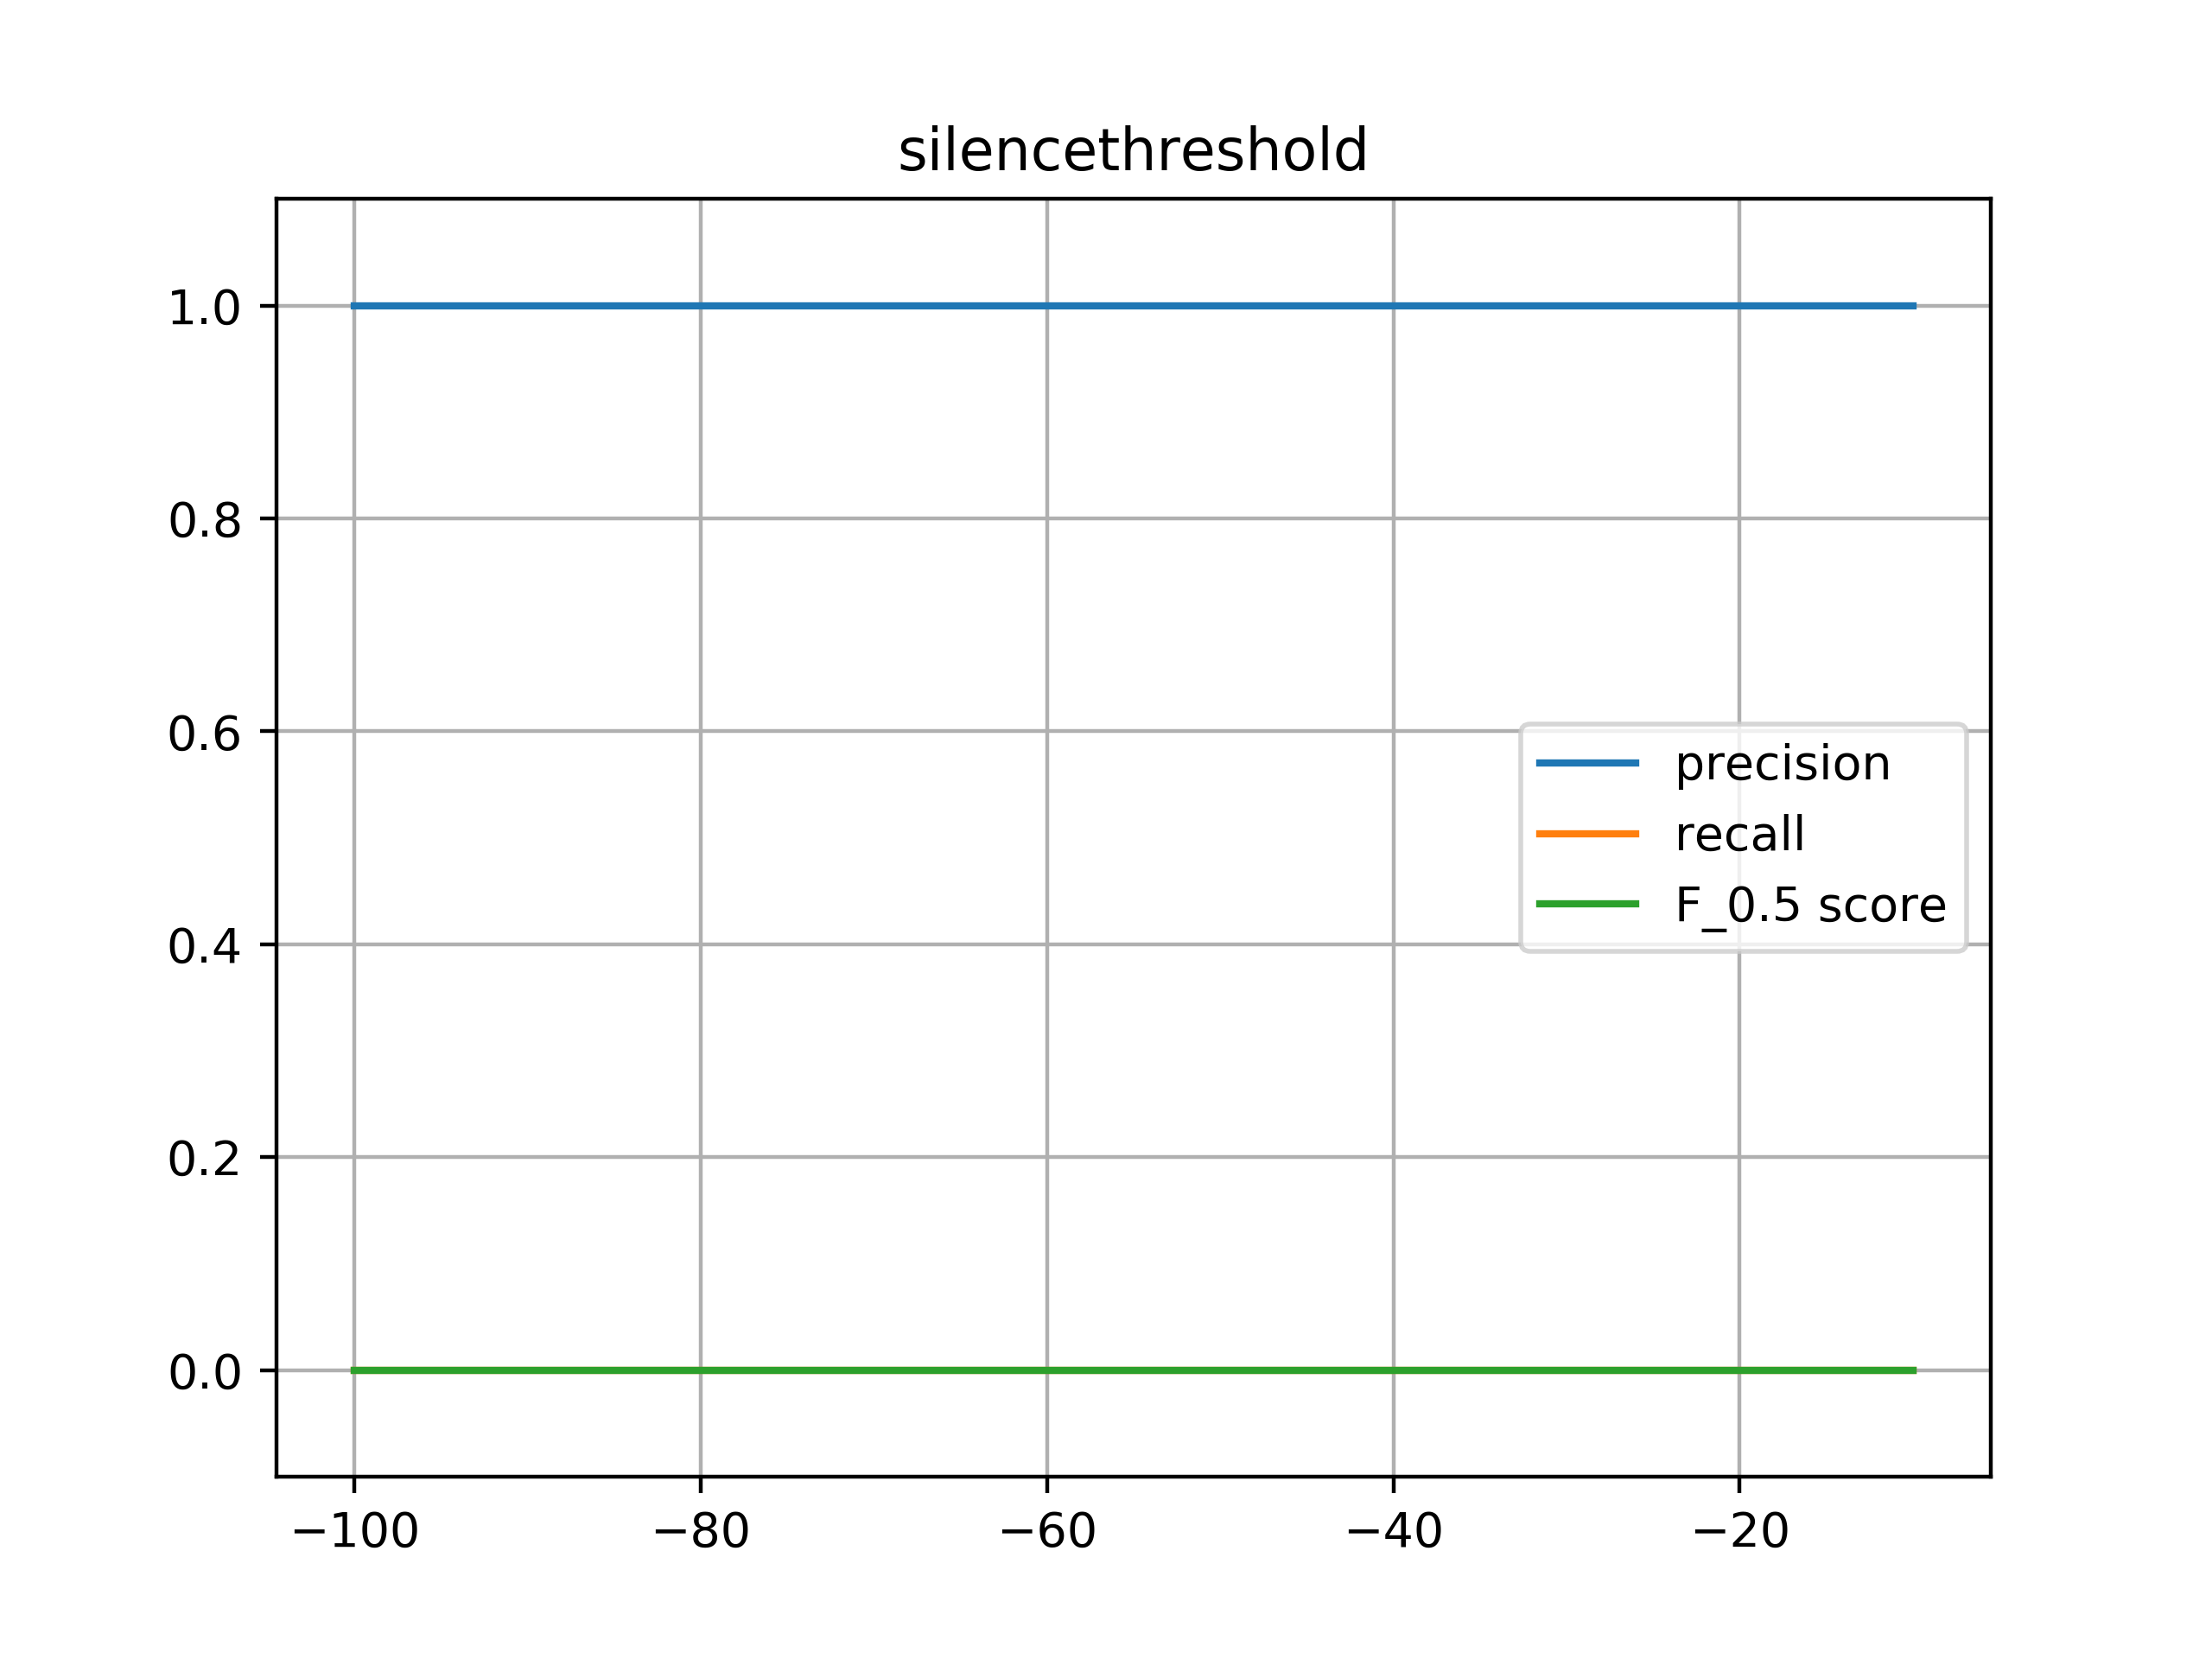
\includegraphics[clip,width=\columnwidth]{Figures/silencethreshold.png}% 
	\caption{threshold parameter sweep results (accuracy, F score and recall)}
	\label{fig:silencethreshold}
\end{figure}

\newpage


